% Options for packages loaded elsewhere
\PassOptionsToPackage{unicode}{hyperref}
\PassOptionsToPackage{hyphens}{url}
\documentclass[
  11pt,
]{article}
\usepackage{xcolor}
\usepackage[margin=22mm]{geometry}
\usepackage{amsmath,amssymb}
\setcounter{secnumdepth}{-\maxdimen} % remove section numbering
\usepackage{iftex}
\ifPDFTeX
  \usepackage[T1]{fontenc}
  \usepackage[utf8]{inputenc}
  \usepackage{textcomp} % provide euro and other symbols
\else % if luatex or xetex
  \usepackage{unicode-math} % this also loads fontspec
  \defaultfontfeatures{Scale=MatchLowercase}
  \defaultfontfeatures[\rmfamily]{Ligatures=TeX,Scale=1}
\fi
\usepackage{lmodern}
\ifPDFTeX\else
  % xetex/luatex font selection
\fi
% Use upquote if available, for straight quotes in verbatim environments
\IfFileExists{upquote.sty}{\usepackage{upquote}}{}
\IfFileExists{microtype.sty}{% use microtype if available
  \usepackage[]{microtype}
  \UseMicrotypeSet[protrusion]{basicmath} % disable protrusion for tt fonts
}{}
\makeatletter
\@ifundefined{KOMAClassName}{% if non-KOMA class
  \IfFileExists{parskip.sty}{%
    \usepackage{parskip}
  }{% else
    \setlength{\parindent}{0pt}
    \setlength{\parskip}{6pt plus 2pt minus 1pt}}
}{% if KOMA class
  \KOMAoptions{parskip=half}}
\makeatother
\usepackage{graphicx}
\makeatletter
\newsavebox\pandoc@box
\newcommand*\pandocbounded[1]{% scales image to fit in text height/width
  \sbox\pandoc@box{#1}%
  \Gscale@div\@tempa{\textheight}{\dimexpr\ht\pandoc@box+\dp\pandoc@box\relax}%
  \Gscale@div\@tempb{\linewidth}{\wd\pandoc@box}%
  \ifdim\@tempb\p@<\@tempa\p@\let\@tempa\@tempb\fi% select the smaller of both
  \ifdim\@tempa\p@<\p@\scalebox{\@tempa}{\usebox\pandoc@box}%
  \else\usebox{\pandoc@box}%
  \fi%
}
% Set default figure placement to htbp
\def\fps@figure{htbp}
\makeatother
\setlength{\emergencystretch}{3em} % prevent overfull lines
\providecommand{\tightlist}{%
  \setlength{\itemsep}{0pt}\setlength{\parskip}{0pt}}
\usepackage{bookmark}
\IfFileExists{xurl.sty}{\usepackage{xurl}}{} % add URL line breaks if available
\urlstyle{same}
\hypersetup{
  hidelinks,
  pdfcreator={LaTeX via pandoc}}

\author{}
\date{}

\begin{document}

\section{Positivity through a moving family of scalar
probes}\label{positivity-through-a-moving-family-of-scalar-probes}

A nonnegative function of position and frequency need not give a
nonnegative operator under left quantization. We construct a positive
operator by testing the symbol against translated, modulated and dilated
scalar probes. The construction works with an arbitrary Hilbert space as
its coefficient space. Its accuracy comes from two separate facts: the
probe has no odd moments, and its scale changes slowly across its
frequency window. Keeping those facts separate also identifies the error
when frequency and position derivatives have equal costs.

The Fourier convention is
\(\widehat u(\xi)=\int e^{-ix\cdot\xi}u(x)\,dx\), with inverse
coefficient \((2\pi)^{-n}\), and \(D=-i\partial\). Fourier inversion and
Plancherel were proved in \href{prerequisite-bridges.pdf}{Fourier
transforms, finite spectra and convex separation}. We use completeness
of Banach spaces, the norm inequality and dominated convergence for
Bochner integrals, scalar Lebesgue integration and Tonelli's theorem,
Taylor's formula, smooth compact cutoffs, and the Hahn--Banach norm
identity \(\|v\|=\sup_{\|\ell\|\leq1}|\ell(v)|\). The Banach-space
completeness and Hahn--Banach steps needed below are in
\href{banach-foundation-bridges.pdf}{Banach estimates, quotient spaces
and compact parameter arguments}; Sections 17--21 of that chapter supply
strong measurability, the full Banach-valued integral and convergence,
both absolute Fubini orders, complete Hilbert-valued L2, the original
monomial Schwartz entry and exact lattice cutoffs, with their original
norms and factors. The scalar symbol estimates imported from
\href{euclidean-symbol-calculus.pdf}{Symbols, operators and Sobolev
scales} are Sections 1--8 of
\href{euclidean-symbol-calculus.pdf}{Symbols, operators and Sobolev
scales}, whose quantization and composition arguments use
\href{gauss-transform-estimates.pdf}{Quadratic Fourier multipliers at a
moving scale}, Sections 7--8 of
\href{gauss-transform-estimates.pdf}{Quadratic Fourier multipliers at a
moving scale}. We prove the necessary Banach and Hilbert space
extensions below; no finite-dimensional approximation of an
operator-valued symbol is assumed.

\subsection{1. Banach coefficients and distributional
duals}\label{banach-coefficients-and-distributional-duals}

Let \(B\) be a complex Banach space. The space
\(\mathcal S(\mathbb R^n;B)\) consists of norm-smooth functions with
finite seminorms \[
 s_N(u)=\max_{|\alpha|\leq N}\sup_x
 \langle x\rangle^N\|\partial^\alpha u(x)\|_B,
 \qquad N=0,1,\ldots.
\tag{P1}
\] All integrals defining their Fourier transforms are Bochner
integrals. Integration by parts gives the usual derivative and
coordinate identities, with convergence in the Banach norm. Fourier
inversion follows by applying every \(\ell\in B'\), using scalar
inversion, and using norm separation to identify the two Banach vectors.
The scalar estimates for Fourier transformation in Schwartz seminorms
give the corresponding norm estimates by the same argument. Completeness
follows by taking the uniform limits of all derivatives on compact sets
and then passing to each weighted bound in (P1).

Use the complex bilinear evaluation \(\langle v,\ell\rangle=\ell(v)\)
for Banach duality. For a reflexive \(B\), define \[
 \mathcal S'(\mathbb R^n;B)
 =\bigl(\mathcal S(\mathbb R^n;B')\bigr)',
\tag{P2}
\] with the topology of uniform convergence on bounded sets of test
functions. Regular functions of polynomial growth act by integration of
this bilinear pairing. This convention has the usual interpretation as
continuous linear maps \(U:\mathcal S(\mathbb R^n)\to B\). Here is an
explicit justification, which will also prevent an incorrect dual space
from entering the transpose construction.

If \(F\) is a functional in (P2), then \(\ell\mapsto F(f\ell)\) is a
bounded linear functional on \(B'\). Reflexivity identifies it with a
unique \(U(f)\in B\). An estimate \(|F(v)|\leq Cs_N(v)\) implies
\(\|U(f)\|\leq Cs_N(f)\), so \(U\) is continuous. Conversely, suppose
\(\|U(f)\|\leq Cs_N(f)\). Choose a smooth lattice partition
\(\sum_{k\in\mathbb Z^n}\chi(x-k)=1\), with \(\chi\) supported strictly
inside a fixed cube. Choose a larger cube of side \(L\) and a cutoff
\(\theta\), supported in its interior and equal to one on
\(\operatorname{supp}\chi\). Fourier expansion on that larger cube
gives, for \(v\in\mathcal S(B')\), \[
 v(x)=\sum_{k,l\in\mathbb Z^n}f_{kl}(x)c_{kl},\qquad
 f_{kl}(x)=\theta(x-k)e^{2\pi i l\cdot(x-k)/L}.
\tag{P3}
\] The coefficients are those of \(\chi(\cdot-k)v\) on the cube centered
at \(k\). We justify the periodic reconstruction used here. On the
circle of period \(L\), with normalized measure \(dt/L\), set \[
 K_N(t)=\frac1N\left|\sum_{j=0}^{N-1}e^{2\pi ijt/L}\right|^2.
\] This kernel is nonnegative and has integral one, since the
exponentials are orthogonal. The geometric-sum formula bounds \(K_N(t)\)
by \(1/(N\sin^2(\pi t/L))\) away from multiples of \(L\). Hence its mass
outside any fixed neighborhood of zero is \(O(N^{-1})\). The product of
these kernels in \(n\) coordinates has integral one and the same
concentration property: outside a small product neighborhood at least
one coordinate is separated from zero, and integration in the other
coordinates leaves unit mass. For a continuous periodic scalar function
\(h\), split its convolution error into that neighborhood and its
complement. Uniform continuity makes the first part arbitrarily small,
and the second is bounded by \(2\|h\|_\infty\) times a mass tending to
zero. Thus these product convolutions converge uniformly to \(h\).

If \(h\) is smooth, periodic integration by parts with \((1-\Delta)^m\)
gives \(|\widehat h(l)|\leq C_m\langle l\rangle^{-2m}\), so its Fourier
series and every differentiated series converge absolutely and
uniformly. Expanding the finite kernel sum shows that the product
convolution has coefficients
\(\widehat h(l)\prod_{j=1}^n(1-|l_j|/N)_+\), where \(r_+=\max(r,0)\).
These factors are bounded by one and tend to one for each fixed \(l\).
Absolute convergence therefore makes the convolutions converge uniformly
to the Fourier sum too. This identifies that sum with \(h\), and
applying the same argument to each derivative gives smooth
reconstruction.

For fixed \(k\), the function \(\chi(\cdot-k)v\) vanishes near the
cube's boundary and thus extends smoothly and periodically. Bochner
integration by parts gives the same norm decay of its coefficients, so
their series and all differentiated series converge absolutely in
\(B'\), uniformly on the cube. Applying every \(\ell\in(B')'\) commutes
with the coefficients and the sums; scalar reconstruction identifies
each scalarized sum with \(\ell(\chi(\cdot-k)v)\). Hahn--Banach norm
separation identifies the Banach vectors themselves. Multiplication by
\(\theta\) therefore recovers exactly \(\chi(\cdot-k)v\). More
quantitatively, Bochner integration by parts shows that for every
\(M,K\), \[
 \|c_{kl}\|_{B'}\leq C_{M,K}s_{M+2K+n}(v)
 \langle k\rangle^{-M}\langle l\rangle^{-2K},
 \qquad
 s_N(f_{kl})\leq C_N\langle k\rangle^N\langle l\rangle^N.
\tag{P4}
\] Choose \(M>N+n\) and \(2K>N+n\). The series
\(\sum_{k,l}\langle U(f_{kl}),c_{kl}\rangle\) converges absolutely and
is bounded by one Schwartz seminorm of \(v\). It defines \(F(v)\). For
each fixed output seminorm, the same estimates with larger \(M,K\) prove
convergence of (P3) in that seminorm. Thus finite sums of scalar test
functions times fixed Banach vectors are dense in \(\mathcal S(B')\).
This proves independence of the partition and uniqueness, since the
functional is prescribed on all such finite sums. The two constructions
are inverse. In the absence of reflexivity, the first construction would
yield \(B''\)-valued maps; that is the reason for the reflexivity
hypothesis in (P2).

Let \(B_1,B_2\) be reflexive, and let \(a\) be a norm-smooth function
with values in \(\mathcal L(B_1,B_2)\). Fix \[
 0<\rho\leq1,\quad 0\leq\delta<1,\quad \delta\leq\rho,
 \qquad \kappa=\rho-\delta.
\tag{P5}
\]

\textbf{Proved extension to real parameters.} Keep (P5) identifiable as
the original range. The calculus, Hilbert bound, moving-probe
construction, moment estimate and lower bound below also hold for \[
 \rho,\delta\in\mathbb R,\qquad\delta\leq\rho\leq1,\qquad\delta<1,
 \qquad\kappa=\rho-\delta\geq0.
 \tag{P5e}
\] There is no lower bound on either parameter. We use the same
seminorms, Fourier convention, ordered coefficient products and original
window; the additional arguments are identified below. Constants may
depend on these fixed real parameters. The classical refinements (P10),
(P43), (P48) and Section 7 retain their classical scope. This is an
extension of this lesson's statement, without a novelty claim. It does
not identify an undated comparison source with the dated edition in the
references. Membership in \(S^r_{\rho,\delta}(B_1,B_2)\) means that \[
 p_{r,N}(a)=\max_{|\alpha|+|\beta|\leq N}
 \sup_{x,\xi}\langle\xi\rangle^{-r+\rho|\alpha|-\delta|\beta|}
 \|\partial_\xi^\alpha\partial_x^\beta a(x,\xi)\|<\infty.
\tag{P6}
\] Write \(S^r=S^r_{1,0}\). These bounds are global in the position
variable. Left quantization is \[
 \operatorname{Op}(a)u(x)=(2\pi)^{-n}
 \int e^{ix\cdot\xi}a(x,\xi)\widehat u(\xi)\,d\xi.
\tag{P7}
\] Norm integration and the product rule prove continuity
\(\mathcal S(B_1)\to\mathcal S(B_2)\): output derivatives introduce only
polynomial factors and symbol derivatives, while powers of \(x\) are
removed by frequency integration by parts. Each output seminorm is
bounded by finitely many seminorms of \(a\) times one sufficiently large
seminorm of \(u\). This Schwartz action in fact holds without
\(\delta\leq\rho\); that restriction is needed for the calculus used
next.

\subsection{2. Ordered products in Banach operator
norm}\label{ordered-products-in-banach-operator-norm}

The symbol product retains the order of its factors. If \(a\) takes
\(B_2\) to \(B_3\) and \(b\) takes \(B_1\) to \(B_2\), then \[
 \operatorname{Op}(a)\operatorname{Op}(b)=\operatorname{Op}(a\circ b),
 \qquad a\circ b\in S^{r+t}_{\rho,\delta}(B_1,B_3),
\tag{P8}
\] and for every integer \(N\geq0\), \[
 a\circ b-\sum_{|\alpha|<N}
 \frac{(\partial_\xi^\alpha a)(D_x^\alpha b)}{\alpha!}
 \in S^{r+t-N\kappa}_{\rho,\delta}(B_1,B_3).
\tag{P9}
\] The maps in (P8)--(P9) are continuous in the seminorms (P6). In the
classical case the stronger estimate before restricting the two pairs of
variables to the diagonal is also valid: in the notation
\(\mathcal B(x,\xi,y,\eta)\) of Section 4 of
\href{euclidean-symbol-calculus.pdf}{Symbols, operators and Sobolev
scales}, the remainder after \(N\) terms obeys \[
 \|\partial_\xi^\alpha\partial_x^\beta
 \partial_\eta^{\alpha'}\partial_y^{\beta'}R_N\|
 \leq C\langle\eta\rangle^{r-N-|\alpha'|}
          \langle\xi\rangle^{t-|\alpha|}.
\tag{P10}
\]

We justify the extension rather than inferring it from a matrix formula.
A scalar linear estimate \(p(Tf)\leq C\sum_jq_j(f)\), when its seminorms
are weighted suprema of finitely many derivatives, extends to
Banach-valued functions by applying \(\ell\in E'\) of norm at most one
and taking the supremum. The Bochner integral definitions commute with
\(\ell\). For the cutoff limits in the Gauss estimates Sections 7--8 of
\href{gauss-transform-estimates.pdf}{Quadratic Fourier multipliers at a
moving scale}, the scalar bounds for the difference of two cutoffs
therefore give Cauchy convergence in the Banach norm, on every compact
set with each derivative. Completeness provides the limit in \(E\); its
scalarizations are exactly the scalar limits. This applies even when
\(E=\mathcal L(B_1,B_3)\) is not reflexive.

Apply that observation to the quadratic multiplier used in Section 4 of
\href{euclidean-symbol-calculus.pdf}{Symbols, operators and Sobolev
scales}, with the Banach-valued input \(a(x,\eta)b(y,\xi)\). Every input
derivative is a finite sum of products in this fixed order and is
bounded by the product of the two relevant operator norms. The metric
and weight calculation in that unit consequently gives (P9) and (P10),
with exactly the same exponent losses. Differentiation before the
diagonal restriction gives each seminorm in (P6). For compactly
supported smooth symbols, Bochner Fubini proves the operator identity
from its absolutely convergent integral kernel. Smooth cutoffs give
bounded approximants converging locally with all derivatives. The
Schwartz estimates for (P7), local convergence, and one extra position
weight prove convergence on each Schwartz input in every output Schwartz
seminorm. Passing to the limit proves (P8). Thus no approximation by
finite-rank operators, and no norm density of finite-rank operators,
enters the proof.

\textbf{Receiving the real-parameter extension.} For (P5e), use exactly
\[
 \begin{split}
 g_{(x,\xi)}(y,\eta)&=\langle\xi\rangle^{2\delta}|y|^2
                 +\langle\xi\rangle^{-2\rho}|\eta|^2,\\
 g_{(x,\xi)}^\sigma(y,\eta)&=\langle\xi\rangle^{2\rho}|y|^2
                 +\langle\xi\rangle^{-2\delta}|\eta|^2,\\
 h(x,\xi)&=\langle\xi\rangle^{\delta-\rho},\qquad
 m_r(x,\xi)=\langle\xi\rangle^r.
 \end{split}
 \tag{P8e}
\] Equations WX1--WX12 in
\href{weyl-metric-products.pdf\#section*.99}{the
full original-metric calculation} prove slow variation, both ordered
temperateness comparisons, local weight continuity and temperateness of
every real-order weight. They also prove uncertainty and the exact
coordinate/directional symbol comparison, with its finite dimension
factors. The metric is unchanged and is invariant under reversal of a
tangent frequency direction. The superscript on its symplectic dual
denotes that dual operation; it is separate from the window exponent
introduced in (P28).

The one-metric Weyl product in
\href{weyl-metric-products.pdf\#section*.72}{Section
7} has cross parameter exactly the displayed \(h\) and remainder weight
\(m_rm_th^N\). The actual Weyl phase retains its factor \(1/4\), and the
induced diagonal metric retains its derivative comparison \(2^{l/2}\) at
order \(l\). Apply the norm-separation construction above to its
localized Gauss series with input \(a(Y)b(Z)\): each finite product-rule
term has that coefficient order, and the summable scalar majorant bounds
its Banach norm. Completeness gives the Banach-valued sum and each
differentiated sum. Thus the full Weyl estimates, bounded-set
local-smooth continuity and all finite remainders hold without
finite-rank approximation.

For the quantization change, the actual phase \(kp\cdot q\), for fixed
\(k\ne0\), has dual \(4k^{-2}g^\sigma\) and parameter \((|k|/2)h\).
Equations WQ1--WQ5 of
\href{weyl-metric-products.pdf\#section*.88}{Section
8} and A35a--A43 of
\href{weyl-covariance-action.pdf\#section*.49}{the
full conversion proof} therefore give the norm-valued map
\(T_k=\exp(ik\langle D_x,D_\xi\rangle)\). Its remainder retains
\((|k|/2)^Nh^N\), the finite counting factor \((1+|k|/2)^{2n}\), and
every actual phase-dependent temperateness constant. At \(k=0\) it is
the identity, with zero remainder for \(N\geq1\) and identity remainder
for \(N=0\). The kernel change and commuting differential-phase identity
in
\href{weyl-covariance-action.pdf\#section*.59}{Section
8} give, in the original coefficient order, \[
 a\circ b=T_{1/2}\big((T_{-1/2}a)\#(T_{-1/2}b)\big),
 \qquad m_rm_th^N=\langle\xi\rangle^{r+t-N\kappa}.
 \tag{P9e}
\] Expand the three conversion maps and the middle Weyl product through
degree \(N-1\). A degree \(j\) coefficient has its proved factor
\(h^j\); every discarded finite term has at least \(h^N\), since
\(h\leq1\). The commuting scalar phases combine exactly to
\(\langle D_\xi,D_y\rangle\), so the retained coefficients are precisely
those of (P9), including \(1/\alpha!\). For \(N=0\) the sum is empty and
the continuous product itself gives the asserted class. This proves
(P8)--(P9) in the extended range.

Use the actual adapted partition in
\href{metric-localization.pdf\#section*.28}{Approximation
on compact sets}: \(a_N=\sum_{\nu\leq N}\phi_\nu a\), and the
corresponding sums for \(b\). At every point at most the fixed overlap
number of supports meet; the full product rule and the original
partition derivative bounds give uniform directional seminorm bounds for
all these finite sums. On any compact set, once its finitely many
meeting supports are included, the sum equals the symbol on a
neighborhood. This proves exactly bounded local-smooth convergence. A
position cutoff independent of frequency need not obey the required
bounds when \(\delta<0\), so it is not used for this passage. The
argument for (P7) uses only finitely many polynomial frequency powers
for each prescribed output seminorm, and so also proves the Schwartz
action for negative parameters. On compact output sets use dominated
frequency integration and local symbol convergence; a common extra
output position weight makes the remaining tails uniformly small. This
passes the compact-symbol operator identity to every Schwartz input.

The reflected base frequency in (P11) preserves all bracket weights.
Kernel transposition and the same \(T_1\) conversion give every original
transpose coefficient and remainder. Equation (P12), the reflexive
identification in Section 1 and the bounded-test estimate then give the
stated strong distribution action. Conjugate kernel transposition gives
(P13), with the original Hilbert pairing and no reflected frequency in
its adjoint symbol. Hence (P8)--(P13) hold under (P5e); (P10) is still
the specified classical estimate. No later positivity or
operator-summation theorem is used as a prerequisite.

For a Banach operator \(A:B_1\to B_2\), let
\(A^{\mathrm t}:B_2'\to B_1'\) be its bilinear transpose. Define
\(c(x,\xi)=a(x,-\xi)^{\mathrm t}\). Transposing the kernel in (P7) gives
right quantization of \(c\). The right-to-left conversion of Section 5
of \href{euclidean-symbol-calculus.pdf}{Symbols, operators and Sobolev
scales}, extended by the scalarization argument just given, supplies a
symbol \(a^{\mathrm T}\in S^r_{\rho,\delta}(B_2',B_1')\) with \[
 a^{\mathrm T}-\sum_{|\alpha|<N}
 \frac{\partial_\xi^\alpha D_x^\alpha c}{\alpha!}
 \in S^{r-N\kappa}_{\rho,\delta}(B_2',B_1').
\tag{P11}
\] In particular the transpose operates on \(B_2'\)-valued tests and
produces \(B_1'\)-valued tests. Define the distributional action by \[
 \langle\operatorname{Op}(a)u,v\rangle
 =\langle u,\operatorname{Op}(a^{\mathrm T})v\rangle,
 \qquad v\in\mathcal S(B_2').
\tag{P12}
\] The right side is continuous in \(v\), and maps bounded sets of tests
to bounded sets, so the resulting map
\(\mathcal S'(B_1)\to\mathcal S'(B_2)\) is continuous for (P2). Kernel
transposition verifies agreement with (P7) on regular Schwartz
distributions. Transposing twice recovers the original kernel;
transposing a product reverses its order. Therefore (P8) holds on
distributions as well. These identities follow first on compact symbol
cutoffs and then by the same distributional convergence; they do not
require density of Schwartz functions in the strong dual topology.

For Hilbert spaces use the inner product linear in its first entry and
let \(a^*\) denote the pointwise Hilbert adjoint. Its formal adjoint
symbol satisfies \[
 a^\dagger-\sum_{|\alpha|<N}
 \frac{\partial_\xi^\alpha D_x^\alpha(a^*)}{\alpha!}
 \in S^{r-N\kappa}_{\rho,\delta},
 \qquad \operatorname{Op}(a)^*|_{\mathcal S}
 =\operatorname{Op}(a^\dagger)|_{\mathcal S}.
\tag{P13}
\] This follows either by conjugating (P11) under the Hilbert dual
identification or directly by conjugate-transposing the kernel. In (P11)
there is a reflected frequency and no conjugation; in (P13) there is
conjugation and no reflected frequency. Keeping these conventions
distinct is essential for distributional targets and signs.

At \(\rho=\delta\), the product and adjoint still belong to the asserted
spaces and every finite remainder estimate remains true, but (P9) and
(P13) give no decrease in order. They are not asymptotic expansions with
a vanishing-order tail at this endpoint.

\subsection{3. Hilbert boundedness independent of
dimension}\label{hilbert-boundedness-independent-of-dimension}

For arbitrary complex Hilbert spaces \(H_1,H_2\), \[
 a\in S^r_{\rho,\delta}(H_1,H_2)
 \quad\Longrightarrow\quad
 \operatorname{Op}(a):H^s(\mathbb R^n;H_1)
 \longrightarrow H^{s-r}(\mathbb R^n;H_2)
 \quad(s\in\mathbb R),
\tag{P14}
\] under (P5e), which includes (P5). The norm is bounded by
\(Cp_{r,L}(a)\), for a finite \(L\) and constants depending on the
displayed parameters and \(n\), not on the dimensions of the Hilbert
spaces. The Sobolev norm is \[
 \|u\|_{H^s(H)}^2=(2\pi)^{-n}
 \int\langle\xi\rangle^{2s}\|\widehat u(\xi)\|_H^2\,d\xi.
\tag{P15}
\] Hilbert-valued Plancherel follows first for functions taking values
in a finite-dimensional span, by an orthonormal basis and scalar
Plancherel. Finite-valued simple functions are dense in Bochner
\(L^2(H)\). Approximating their scalar components by Schwartz functions
and taking the isometric completion proves Plancherel and Schwartz
density for all \(H\), including nonseparable \(H\). This uses only
strong measurability; every particular Bochner function is almost
everywhere valued in some separable closed subspace.

Here are the analytic estimates behind (P14). If
\(K(X,Y)\in\mathcal L(H_1,H_2)\) has both marginal integrals of its
operator norm bounded by \(C\), then \[
 \left\|\int K(X,Y)f(Y)\,dY\right\|^2
 \leq\left(\int\|K(X,Y)\|\,dY\right)
       \left(\int\|K(X,Y)\|\|f(Y)\|^2\,dY\right).
\tag{P16}
\] Integration in \(X\) proves the norm bound \(C\). Truncation and
completion define the operator when necessary. This estimate uses the
norm of the actual vector input, not a sum over a basis of the
coefficient space.

\textbf{Editorial clarification: the actual measurable kernel and its
Hilbert receiving map.} Equation (P16) uses a Bochner integral. Its
general kernel statement requires measurability of that vector integrand
as well as the displayed norm marginal bounds. The actual packet kernel
below has this property. We prove both its precise integral construction
and its comparison with a more general canonical kernel map, including
the nonseparable case.

Let \((X,\mu)\), \((Y,\nu)\) be the original sigma-finite Euclidean
measure spaces in the application, and retain complex Hilbert spaces
\(H_1,H_2\), with inner products linear in the first entry. Suppose
\(K(x,y):H_1\to H_2\) is weakly operator measurable:
\(\langle K(x,y)h,k\rangle\) is measurable for every fixed \(h,k\).
Assume separately that \(k_0(x,y)=\|K(x,y)\|\) is measurable and that
its actual marginals satisfy \[
\int_Yk_0(x,y)\,d\nu(y)\le A\quad\text{for a.e. }x,
\qquad \int_Xk_0(x,y)\,d\mu(x)\le B\quad\text{for a.e. }y,
\tag{HM1}
\] with finite \(A,B\ge0\). The measures and both constants remain
separate. For Bochner \(L^2\) inputs \(f\) and \(g\), approximation by
strongly measurable simple functions shows that
\(\langle K(x,y)f(y),g(x)\rangle\) is measurable on the original
product: for each simple pair it is a countable sum of the prescribed
measurable scalar pairings, and the pointwise limit gives the full
pairing. Product null sets caused by representatives are null by
sigma-finiteness and Tonelli. Weighted Cauchy--Schwarz on this original
product gives \[
\begin{aligned}
\iint k_0(x,y)\|f(y)\|\|g(x)\|\,d\nu(y)d\mu(x)
&\le\left(\iint k_0(x,y)\|f(y)\|^2\,d\nu(y)d\mu(x)\right)^{1/2}\\
&\quad{}\times\left(\iint k_0(x,y)\|g(x)\|^2\,d\nu(y)d\mu(x)\right)^{1/2}\\
&\le\sqrt{AB}\,\|f\|_{L^2(\nu;H_1)}\|g\|_{L^2(\mu;H_2)}.
\end{aligned}
\tag{HM2}
\] Thus the scalar integral \(b_K(f,g)\) of the original pairing is
absolutely convergent, independent of representatives, linear in \(f\),
and conjugate-linear in \(g\). The complete Hilbert representation
theorem gives a unique element \(T_Kf\in L^2(\mu;H_2)\) with \[
\langle T_Kf,g\rangle=b_K(f,g),\qquad
\|T_K\|\le\sqrt{AB}.
\tag{HM3}
\] Uniqueness proves linearity in \(f\) and in the kernel. This is an
actual bounded map on the original Bochner Hilbert spaces, even when a
pointwise vector integral has not been constructed. If either marginal
constant is zero, (HM2) makes the pairing and operator zero, with no
division by that constant. The swapped kernel \(K^\star(y,x)=K(x,y)^*\)
is weakly operator measurable, its norm is unchanged, and its marginal
constants are \(B,A\). Absolute scalar Fubini, retaining the conjugation
convention, gives \(T_{K^\star}=T_K^*\).

Now impose the extra strong-action hypothesis that
\((x,y)\mapsto K(x,y)h\) is strongly measurable for every fixed
\(h\in H_1\). Simple approximation to \(f\) and pointwise norm
convergence prove strong measurability of \(F(x,y)=K(x,y)f(y)\). For
almost every \(x\), the second squared integral in (P16), in its
original order, is finite by Tonelli and the column bound. The row bound
and scalar Cauchy--Schwarz give \(\int\|F(x,y)\|d\nu(y)<\infty\).
Sections of the strongly measurable product function are strongly
measurable for almost every \(x\), by countable simple approximants and
scalar Fubini on their exceptional sets. Therefore the Bochner integral
exists there. On every finite-measure piece \(E\subset X\), (HM2)
applied to the nonnegative scalar input \(1_E(x)\) bounds
\(\int_{E\times Y}\|F\|\) by \(\sqrt{AB}\|f\|_2\mu(E)^{1/2}\). Bochner
Fubini on these pieces, then their sigma-finite exhaustion, proves that
\[
v(x)=\int_YK(x,y)f(y)\,d\nu(y)
\quad\text{is strongly measurable,}\qquad
\|v\|_2^2\le AB\|f\|_2^2.
\tag{HM4}
\] Pairing this actual \(v\) with any \(g\), the full absolutely
convergent pairing (HM2) and Bochner integration give
\(\langle v,g\rangle=b_K(f,g)\). Uniqueness in (HM3) proves \(v=T_Kf\)
as the original \(L^2\) class. Thus (P16)'s vector integral is exactly
the canonical map when its strong-action hypothesis holds. Its original
common-bound case is \(A=B=C\), giving norm at most \(C\).

Here is why the hypothesis cannot be inferred from norm bounds in an
arbitrary nonseparable coefficient space. Take the original Lebesgue
spaces \(X=Y=(0,1)\), \(H_1=\mathbb C\), \(H_2=\ell^2((0,1))\), and let
\(e_y\) be the unit vector at index \(y\). Put \(K(x,y)z=ze_y\). Its
norm is one, so both original marginals are exactly one. Every vector in
\(\ell^2((0,1))\) has countable support: for each positive integer
\(j\), only finitely many coordinates can have absolute value at least
\(1/j\), by its finite squared norm; the support is the countable union
of those sets. Therefore each fixed scalar pairing with \(e_y\) is
supported on a countable set and is measurable, so \(K\) satisfies
(HM1)--(HM3). But \(y\mapsto e_y\) is not strongly measurable. Any
separable subspace has a countable dense family, whose supports have
countable union \(S\); every vector in the subspace is supported on
\(S\), by norm convergence of the dense family. Outside \(S\), the unit
vector \(e_y\) does not belong to that subspace. This contradicts the
a.e. separable range of a strongly measurable function, since \(S\) has
Lebesgue measure zero. Hence (P16)'s Bochner integral for the constant
input one cannot be formed for this kernel.

Nevertheless its exact canonical map exists and is zero. A Bochner
\(L^2\) test \(g(x)\) is a.e. valued in a separable subspace, by its
simple approximants. The preceding support argument gives one countable
set \(S\) supporting all those values. Thus
\(\langle K(x,y)f(y),g(x)\rangle=0\) for almost every pair \((x,y)\),
and (HM3) gives \(T_K=0\). The precise defect defines a kernel space,
rather than an unidentified failure: on the vector space \(\mathfrak K\)
of weakly operator measurable kernels with measurable norm and finite
marginals, set \[
\mathfrak N=\{K\in\mathfrak K:b_K(f,g)=0\text{ for all original }f,g\}.
\tag{HM5}
\] Equation (HM3) proves \(\mathfrak N=\ker(K\mapsto T_K)\).
Consequently \([K]\mapsto T_K\) is an injective linear map from
\(\mathfrak K/\mathfrak N\) to the actual bounded operators; the norm
\(\|[K]\|=\|T_K\|\) is well defined and is zero only on the zero class.
Equation (HM2) gives its exact upper bound by the original marginals.
The exhibited norm-one kernel belongs to \(\mathfrak N\). No
surjectivity or completeness of this quotient is presumed.

For the actual packet kernel (P17b), there is no strong-measurability
defect. The original symbol is norm-smooth in its original Banach
operator space. Its compact-parameter variations in the integral have a
common scalar Schwartz majorant: its zeroth uniform derivative bound and
the factors \(|\widehat g(\zeta)g(z)|\) give an integrable majorant.
Pointwise operator-norm continuity, including the full scalar phase
\(e^{iq\cdot(p'-p)}e^{i[z\cdot(p'-p)+\zeta\cdot(q-q')+z\cdot\zeta]}\),
and Bochner dominated convergence prove operator-norm continuity of
\(K_a\) in every packet parameter. Its operator-valued integrand is
strongly measurable too: a continuous image of the separable Euclidean
parameter domain is separable, and approximation on countably many
compact cubes supplies measurable simple approximants. The same
reasoning applies to every fixed-vector action of \(K_a\) and of its
swapped adjoint; taking an adjoint preserves operator-norm continuity.

The two inverse Fourier factors in that application can be displayed
separately. Set \[
\begin{aligned}
c_\alpha&=\binom N{|\alpha|}\frac{|\alpha|!}{\alpha!}\quad(|\alpha|\le N),\\
R_{\gamma,\delta}(z,\zeta)
 &=\sum_{\substack{\tau\le\delta\\\tau\le\gamma}}
 \binom\delta\tau i^{|\gamma|+|\delta|-|\tau|}
 \frac{\gamma!}{(\gamma-\tau)!}\zeta^{\gamma-\tau}z^{\delta-\tau}.
\end{aligned}
\] The polynomial is exactly
\(e^{-iz\cdot\zeta}\partial_z^\gamma\partial_\zeta^\delta e^{iz\cdot\zeta}\),
by differentiating \((i\zeta)^\gamma e^{iz\cdot\zeta}\) with the full
product rule. The expansion of \((1-\Delta_z)^N\) has coefficient
\((-1)^{|\alpha|}c_\alpha\partial_z^{2\alpha}\); the other operator has
the corresponding \(\beta\) expansion, retaining those signs before
taking absolute values. Define the following finite complete majorant:
\[
\begin{aligned}
C_N(g)={}&\iint\sum_{\substack{|\alpha|\le N\\|\beta|\le N}}c_\alpha c_\beta
 \sum_{\substack{\gamma_1+\gamma_2+\gamma_3=2\alpha\\
                  \delta_1+\delta_2+\delta_3=2\beta}}
 \frac{(2\alpha)!}{\gamma_1!\gamma_2!\gamma_3!}
 \frac{(2\beta)!}{\delta_1!\delta_2!\delta_3!}\\
 &\quad{}\times|R_{\gamma_1,\delta_1}(z,\zeta)|
 |\partial_\zeta^{\delta_3}\widehat g(\zeta)|
 |\partial_z^{\gamma_3}\overline{g(z)}|\,dz\,d\zeta.
\end{aligned}
\] Here the second derivative group acts on the original symbol, and the
first on its exponential; the third groups act on the two scalar
windows. The other cross-window derivatives are exactly zero because
each window depends on only its own variable. Every coefficient, sign,
nonzero term and zero case is therefore accounted for in the original
four-factor product rule. The majorant is finite because each displayed
polynomial times the differentiated windows is integrable. Each
differentiated symbol has total order at most \(4N\), so the original
\(M\) in (P18) bounds its norm. Integration by parts in the original
integral (P17b), with its full constant phase retained, now gives \[
\begin{aligned}
\|K_a(q,p;q',p')\|&\le(2\pi)^{-n}C_N(g)M
       \langle q-q'\rangle^{-2N}\langle p-p'\rangle^{-2N},\\
\int\|K_a\|\,(2\pi)^{-n}dq'\,dp'
 &\le(2\pi)^{-2n}C_N(g)M I_N^2,
 \qquad I_N=\int\langle z\rangle^{-2N}dz.
\end{aligned}
\tag{HM6}
\] The opposite marginal has the same full bound, by integration in
\(q,p\). Retain the exact original measures
\(d\mu=d\nu=(2\pi)^{-n}dq\,dp\); \(I_N\) is finite for the original
\(N>n/2\). Apply (HM4) with both marginals in (HM6). Thus the Bochner
packet operator, its canonical Hilbert operator, and the swapped-adjoint
kernel operator are the exact maps just proved. The packet isometry and
synthesis give the original \(\operatorname{Op}(a)\) on Schwartz inputs.
This verifies the actual use of (P16) on its full nonseparable Hilbert
domain, with both inverse Fourier factors visible and no
coefficient-dimension factor or finite-rank approximation.

Fix a scalar Schwartz function \(g\) of \(L^2\) norm one. The transform
\(Vu(q,p)=\int u(x)\overline{e^{ip\cdot x}g(x-q)}\,dx\) is an isometry
into \(L^2((2\pi)^{-n}dq\,dp;H)\), by Hilbert-valued Plancherel followed
by integration in \(q\). Its synthesis map has norm one and \(V^*V=I\),
by polarization. If all symbol derivatives through order \(4N\) are
uniformly bounded in operator norm, the packet kernel of
\(V\operatorname{Op}(a)V^*\) is an operator-valued version of the double
integral in Section 6 of \href{euclidean-symbol-calculus.pdf}{Symbols,
operators and Sobolev scales}. After writing \(x=q+z\),
\(\xi=p'+\zeta\), its amplitude is \[
 (2\pi)^{-n}e^{iz\cdot\zeta}
 a(q+z,p'+\zeta)\widehat g(\zeta)\overline{g(z)}.
\tag{P17}
\] The integration-variable phase is
\(e^{i[z\cdot(p'-p)+\zeta\cdot(q-q')]}\). Its full constant factor must
also be retained. Write \(g_{q,p}(x)=e^{ip\cdot x}g(x-q)\), keep the
original linear-first pairing and phase-space measure
\((2\pi)^{-n}dq\,dp\), and let \(K_a(q,p;q',p')\) be the operator-valued
packet kernel with that measure. The original forward transform gives
\(\widehat g_{q',p'}(\xi)=e^{-iq'\cdot(\xi-p')}\widehat g(\xi-p')\).
With \(x=q+z\) and \(\xi=p'+\zeta\), the entire exponent is \[
 (q+z)\cdot(p'+\zeta)-q'\cdot\zeta-p\cdot(q+z)
 =q\cdot(p'-p)+z\cdot(p'-p)
                      +\zeta\cdot(q-q')+z\cdot\zeta.
 \tag{P17a}
\] Both coordinate substitutions have Jacobian one. Thus the complete
packet kernel, including every scalar factor and the original
coefficient order, is \[
 \begin{split}
 K_a(q,p;q',p')&=e^{iq\cdot(p'-p)}(2\pi)^{-n}
    \iint e^{i[z\cdot(p'-p)+\zeta\cdot(q-q')]}\\
 &\quad{}\times e^{iz\cdot\zeta}
       a(q+z,p'+\zeta)\widehat g(\zeta)\overline{g(z)}\,dz\,d\zeta.
 \end{split}
 \tag{P17b}
\] The double integral converges in operator norm under the displayed
uniform zeroth symbol bound because both scalar windows are Schwartz.
Applying the original quantization to \(g_{q',p'}h\), pairing with
\(g_{q,p}k\), and using absolute Fubini proves this equality for every
\(h\in H_1\), \(k\in H_2\); separation by these Hilbert pairings
identifies the operator-valued kernel. This is precisely the full scalar
phase of EC12--EC14 in
\href{euclidean-symbol-calculus.pdf\#section*.36}{the
Euclidean lesson}, with its Schwartz window renamed to the original
\(g\). The factor \(e^{iq\cdot(p'-p)}\) has absolute value one for the
real packet parameters and is independent of \(z,\zeta\); it remains
present through all integrations by parts, while the original inverse
Fourier multiplier stays \((2\pi)^{-n}\). Integration by parts with
\((1-\Delta_z)^N(1-\Delta_\zeta)^N\) bounds the kernel norm by \[
 C M\langle q-q'\rangle^{-2N}\langle p-p'\rangle^{-2N},
 \qquad
 M=\max_{|\alpha|+|\beta|\leq4N}
 \|\partial_\xi^\alpha\partial_x^\beta a\|_\infty.
\tag{P18}
\] All polynomial factors created by differentiating the exponential in
(P17) are absorbed by the two scalar Schwartz functions. For \(N>n/2\),
(P16) bounds the packet operator by \(CM\). Reconstruction on Schwartz
inputs proves the same bound for \(\operatorname{Op}(a)\); no prior
\(L^2\) boundedness is used.

For an order-zero symbol under (P5), decompose the frequency variable
into dyadic annuli with cutoffs \(\chi_j\), and set \(a_j=a\chi_j\).
Conjugation by scalar unitary dilation changes the symbol to
\(a_j(2^{-j\rho}X,2^{j\rho}\Xi)\), whose derivatives are uniformly
bounded: a position derivative contributes
\(2^{-j\rho}2^{j\delta}\leq1\), and a frequency derivative contributes
\(2^{j\rho}2^{-j\rho}=1\). Cutoff derivatives obey these bounds because
\(\rho\leq1\). Thus (P18) gives a uniform bound for each piece.

To sum the pieces, use a scalar Schwartz function \(\omega\) with
\(\widehat\omega\) compactly supported, equal to one near zero, and
supported in the unit ball. Its integral is one and all its nonconstant
moments vanish. Convolve \(a_j\) in position at scale
\(\lambda_j=2^{j-4}\), as in \[
 \ell_j(x,\xi)=\int\omega(z)a_j(x-z/\lambda_j,\xi)\,dz,
 \qquad r_j=a_j-\ell_j.
\tag{P19}
\] The norm-valued Taylor formula with \(K\) derivatives gives, for each
fixed pair \(\alpha,\beta\), \[
 \|\partial_\xi^\alpha\partial_x^\beta r_j\|_\infty
 \leq Cp_{0,L}(a)2^{-jK(1-\delta)}
       2^{-j\rho|\alpha|+j\delta|\beta|}.
\tag{P20}
\] After the preceding dilation, (P18) makes the operator norms of the
\(r_j\) summable, since \(\delta<1\). The base Fourier support of
\(\ell_j\) lies in a ball of radius \(2^{j-4}\). Consequently its
operator only receives input in the \(j\)-th frequency annulus and has
output in a fixed enlargement of that annulus. This support statement
follows in the distributional Fourier formula by testing against
disjoint supports; it does not require an operator-valued pointwise
Fourier transform in position. The input annuli and enlarged output
annuli both have bounded overlap. The Hilbert space inequality
\(\|v_1+\cdots+v_k\|^2\leq k\sum\|v_i\|^2\), applied at each output
frequency, and Plancherel show that \[
 \left\|\sum_j\operatorname{Op}(\ell_j)u\right\|_2^2
 \leq Cp_{0,L}(a)^2\sum_j\|P_ju\|_2^2
 \leq Cp_{0,L}(a)^2\|u\|_2^2.
\tag{P21}
\] Here \(P_j\) is the input annulus projection. The tail of the middle
sum tends to zero for each input, proving strong convergence. Adding
(P20) and the single low-frequency term establishes order-zero
boundedness. It includes \(0<\rho=\delta<1\). Finally apply (P8) to
\(\langle D\rangle^{s-r}\operatorname{Op}(a)\langle D\rangle^{-s}\),
whose symbol has order zero. This proves (P14) for all real \(r,s\),
with finite-seminorm control. \(\square\)

\textbf{The same Hilbert proof for negative parameters.} In the
order-zero annular argument, differentiating \(a\chi_j\) gives the
complete terms \[
 {\alpha\choose\gamma}
 (\partial_\xi^{\alpha-\gamma}\partial_x^\beta a)
 (\partial_\xi^\gamma\chi_j),\qquad \gamma\leq\alpha.
 \tag{P21e}
\] For \(j\geq1\) the supports have \(\langle\xi\rangle\) comparable to
\(2^j\) and the cutoff bound is \(C_\gamma2^{-j|\gamma|}\). After the
displayed unitary dilation each term is bounded by its binomial
coefficient times
\(C_\gamma p_{0,L}(a)2^{j(\delta-\rho)|\beta|+j(\rho-1)|\gamma|}\),
which is uniformly bounded for every real pair in (P5e). The change of
coordinates is still unitary even when its scale tends in the other
direction. In (P19), all nonconstant moments still vanish; the integral
Taylor remainder retains \(\lambda_j^{-K}2^{jK\delta}\), including its
fixed factor \(2^{4K}\). This is (P20), and its norms are summable
because \(K(1-\delta)>0\). The unchanged frequency-support argument
proves (P21) with bounded overlap. It uses no sign condition on \(\rho\)
or \(\delta\).

For each real \(v\),
\(\partial_\xi^\alpha\langle\xi\rangle^v=O(\langle\xi\rangle^{v-|\alpha|})\),
and position derivatives vanish. Since \(\rho\leq1\), this scalar
multiplier belongs to \(S^v_{\rho,\delta}\), even when \(\rho\) is
negative. The already proved ordered calculus therefore puts the Sobolev
conjugate in order zero, proving (P14) under (P5e) with linear
finite-seminorm control. This direct annular proof needs neither the
later metric-operator chapter nor the moving-window estimate.

\textbf{Editorial extension: Hilbert-valued Besov maps in the full
signed range.} The endpoint theorem (P14) has a further exact
consequence. For every original Hilbert coefficient space \(H\), retain
the original Fourier convention and sharp annuli \(A_0=\{|\xi|<1\}\),
\(A_j=\{2^{j-1}\le|\xi|<2^j\}\), \(j\ge1\), of
\href{euclidean-symbol-calculus.pdf\#section*.62}{the
Sobolev chapter}. On locally Bochner \(L^2\) Fourier transforms define,
for \(0<p<\infty\), \[
N_{s,p,H}(u)=\left(\sum_{j\ge0}(2^{js}\|\Pi_ju\|_{L^2(H)})^p\right)^{1/p},
\qquad N_{s,\infty,H}(u)=\sup_{j\ge0}2^{js}\|\Pi_ju\|_{L^2(H)}.
\tag{HB1}
\] Here \(\Pi_j\) is the actual sharp Fourier projection and each
Hilbert \(L^2\) norm uses the actual original base measure. The domain
is denoted \(B^s_{2,p}(H)\). For \(p\ge1\) this is a norm; for \(p<1\),
\(d(u,v)=N_{s,p,H}(u-v)^p\) is its translation-invariant metric, by the
scalar inequality proved in BQ2 and the Hilbert norm triangle
inequality.

We identify its full distribution domain. Choose arbitrary Bochner
\(F_j\in L^2(A_j;H)\), extended by zero, with
\(v_j=2^{js}(2\pi)^{-n/2}\|F_j\|_2\) in the indicated sequence space.
Their supports are the original disjoint annuli, and their countably
many essentially separable ranges lie in one separable closed subspace
of \(H\); thus \(F=\sum_jF_j\) is locally strongly measurable and
locally \(L^2\). The inverse Fourier distribution is the actual
\(H\)-valued map \[
U(\varphi)=(2\pi)^{-n}\sum_{j\ge0}
     \int_{A_j}F_j(\xi)\widehat\varphi(-\xi)\,d\xi.
\tag{HB2}
\] Every integral and the series converge in the Hilbert norm. For
\(j\ge1\), retain \(|A_j|\le\omega_n2^{jn}\); with
\(C_L=\sup_\xi\langle\xi\rangle^L|\widehat\varphi(-\xi)|\), the norm of
its full summand is at most
\((2\pi)^{-n/2}\omega_n^{1/2}2^LC_L2^{j(n/2-s-L)}v_j\). Choose an
integer \(L>n/2-s\), and use \(v_j\le N_{s,p,H}\), also for the supremum
case. The complete geometric tail converges; the low term is bounded by
\((2\pi)^{-n/2}v_0\|\widehat\varphi\|_{L^2(A_0)}\). These estimates
prove continuity \(\mathcal S\to H\). The reflexive identification
P2--P4 therefore gives an actual \(H\)-valued tempered distribution,
whose Fourier transform is \(F\), with
\(\|\Pi_ju\|_{L^2(H)}=(2\pi)^{-n/2}\|F_j\|_2\) by the proved Hilbert
Plancherel theorem. Conversely the original locally Bochner \(L^2\)
Fourier pieces of any element reconstruct that same distribution by
(HB2), since the tested tail tends to zero. No extra generalized
elements have been added to the domain.

Completeness follows on this exact domain. For a Cauchy sequence, every
weighted Fourier piece is Cauchy in its actual Hilbert space and has a
limit \(F_j\). For finite \(p\), finite sums and their increasing limit
give \[
\sum_j\left(2^{js}(2\pi)^{-n/2}
 \|F_j-\widehat{\Pi_ju^{(r)}}\|_2\right)^p
\le\liminf_{t\to\infty}N_{s,p,H}(u^{(t)}-u^{(r)})^p.
\tag{HB3}
\] For \(p=\infty\), take the supremum of the individual limits instead;
it is bounded by the same limiting supremum of the Cauchy differences.
One fixed index and the norm or quasi-triangle inequality give a finite
limiting sequence norm. Equation (HB2) constructs its actual
distribution, and (HB3), or the supremum bound, proves convergence in
the original metric or norm. Thus all these spaces are complete.

On every original annulus, \(2^{-j}\langle\xi\rangle\in[1/2,\sqrt2]\),
including the low piece. For real \(t\) put
\(a_t=\min(2^{-t},2^{t/2})\), \(b_t=\max(2^{-t},2^{t/2})\). The original
Sobolev norm (P15) gives \[
\begin{aligned}
a_t2^{jt}\|\Pi_ju\|_{L^2(H)}&\le\|\Pi_ju\|_{H^t(H)}
 \le b_t2^{jt}\|\Pi_ju\|_{L^2(H)},\\
\|u\|_{H^{s_-}(H)}^2&\le
 {b_{s_-}^2\over1-2^{-2(s-s_-)}}N_{s,p,H}(u)^2
 \qquad(s_-<s).
\end{aligned}
\tag{HB4}
\] The second line follows by summing the disjoint original squared
Fourier pieces and bounding each \(v_j\) by its sequence norm. It proves
actual convergence of the annular input partial sums in the lower
endpoint for every \(p\), including infinity.

Let \(T\) be the actual consistent map from \(H^{s_-}(H_1)\) to
\(H^{s_--r}(H_2)\) and from \(H^{s_+}(H_1)\) to \(H^{s_+-r}(H_2)\), with
norms \(M_-,M_+\), where \(s_-<s<s_+\). The first line of (HB4), applied
at both endpoints, gives \[
2^{k(s-r)}\|\Pi_kT\Pi_ju\|_{L^2(H_2)}
\le Cc_{k-j}\,2^{js}\|\Pi_ju\|_{L^2(H_1)},
\quad c_l=\min(2^{l(s-s_-)},2^{l(s-s_+)}),
\tag{HB5}
\] where \(C=\max(M_-b_{s_-}/a_{s_--r},M_+b_{s_+}/a_{s_+-r})\). Every
original Fourier factor is already retained in both Hilbert norms. For
finite annular input sums, apply the target Hilbert triangle inequality
at each \(k\). If \(0<p<1\), raise the scalar sum to \(p\), use
\((a+b)^p\le a^p+b^p\), and then sum over \(k\). If \(1\le p<\infty\),
the \(\ell^p\) triangle inequality for translations gives the
convolution bound; it follows for arbitrary summable nonnegative kernels
by finite sums and their increasing limits. For \(p=\infty\), take the
supremum directly. In all cases the resulting exact bound is \[
N_{s-r,p,H_2}(Tu)\le C D_p N_{s,p,H_1}(u),
\tag{HB6}
\] where \[
\begin{aligned}
D_p^p&=1+{2^{-p(s-s_-)}\over1-2^{-p(s-s_-)}}
          +{2^{-p(s_+-s)}\over1-2^{-p(s_+-s)}}&& (0<p<1),\\
D_p&=1+{2^{-(s-s_-)}\over1-2^{-(s-s_-)}}
          +{2^{-(s_+-s)}\over1-2^{-(s_+-s)}}&& (1\le p\le\infty).
\end{aligned}
\] These are the complete sums on \(\mathbb Z\), with both tails,
central term and positive denominators retained. For an arbitrary input,
(HB4) defines the actual \(Tu\) at the lower endpoint. Its finite
annular input sums converge there, so every fixed target projection
converges in Hilbert \(L^2\), by the positive lower Sobolev weight on
that original annulus. Pass the estimate first to a finite set of output
indices, then to all indices by increasing sums or the supremum. This
proves (HB6) for the actual endpoint operator. It does not require
density of finite annular sums in the infinity Besov norm.

Take \(T=\operatorname{Op}(a)\) from the proved theorem (P14). We have
consequently proved \[
\operatorname{Op}(a):B^s_{2,p}(H_1)\longrightarrow B^{s-r}_{2,p}(H_2)
\quad(0<p\le\infty,\ s,r\in\mathbb R)
\tag{HB7}
\] for every original \(a\in S^r_{\rho,\delta}(H_1,H_2)\) under the
entire signed range (P5e), including \(\rho\le0\) and \(\rho=\delta<1\).
The constants are controlled by finitely many original operator-norm
symbol seminorms and the displayed scalar constants, independently of
both Hilbert dimensions. We have used the proved signed-parameter
Hilbert endpoints, rather than substituting a scalar symbol theorem with
a smaller parameter range.

The original smooth-cutoff comparison is valid on these Hilbert domains
as well. With a smooth partition \(\phi_k\) bounded by \(M\), meeting
\(A_j\) only when \(|j-k|\le L\), the two identities in BQ6 are actual
Hilbert Fourier multiplier identities. For \(p<1\), their complete
bounds are respectively \(M^p2^{p|s|L}(2L+1)\) and \(2^{p|s|L}(2L+1)\)
on the sums of \(p\)-th powers, by the Hilbert triangle inequality
followed by its scalar \(p\)-power bound. For \(p\ge1\), each individual
translation has factor at most \(M2^{|s|L}\) in the forward direction,
and \(2^{|s|L}\) in the reverse direction; summing the at most \(2L+1\)
translations gives these factors times \(2L+1\), including the supremum
endpoint. This proves equivalence to the same smooth dyadic spaces
without a basis or finite-rank argument. In dimension zero only the
original low piece exists; (HB1) is the original Hilbert norm and the
maps are the one-point coefficient maps. These standard editorial
consequences do not assert a Banach-coefficient Plancherel or positivity
theorem and carry no novelty claim.

There is no assertion here that this \(L^2\) theorem holds for arbitrary
reflexive Banach coefficient spaces. The preceding calculus does; the
present proof uses Hilbert-valued Plancherel at its central step.

\subsection{4. A positive scalar probe and its moving
copies}\label{a-positive-scalar-probe-and-its-moving-copies}

Choose an even \(\varphi\in C_c^\infty(\mathbb R^{2n})\) with
\(\|\varphi\|_{L^2(\mathbb R^{2n})}=1\). Even means simultaneous
inversion of both variables. Let \(B=\operatorname{Op}(\varphi)\),
acting on scalar functions. Its kernel is Schwartz. The kernel \[
 K_Q(x,z)=\int\overline{K_B(t,x)}K_B(t,z)\,dt
\tag{P22}
\] is Schwartz as well: differentiate under the integral and use the
rapid decay of the two factors with any desired polynomial weights.
Fourier transformation in \(x-z\) therefore defines a unique
\(\psi\in\mathcal S(\mathbb R^{2n})\) with \[
 \operatorname{Op}(\psi)=B^*B.
\tag{P23}
\] Conjugation by parity \(u(x)\mapsto u(-x)\) fixes \(B\) because
\(\varphi\) is even. It fixes \(B^*B\) too, so uniqueness of the
Schwartz kernel symbol proves that \(\psi\) is even. The function
\(\psi\) need not be real or pointwise nonnegative: the property being
imposed is positivity of its quantization.

The normalization is precisely \[
 \int\psi(x,\xi)\,dx\,d\xi=1.
\tag{P24}
\] Indeed Fourier inversion on the diagonal gives
\((2\pi)^{-n}\int\psi=\int K_Q(x,x)\,dx\). By (P22) the latter equals
\(\iint|K_B(t,x)|^2\,dt\,dx\). Scalar Plancherel in the kernel formula
for \(B\) makes this \((2\pi)^{-n}\|\varphi\|_2^2\). Cancelling the
common factor proves (P24). This computation uses ordinary integrals of
Schwartz kernels, and needs no trace-class theorem.

For \(q>0\) define the scalar unitary \[
 (U_{y,\eta,q}v)(x)=q^{n/2}e^{i\eta\cdot x}v(q(x-y)).
\tag{P25}
\] Changing variables in (P7) gives \[
 U_{y,\eta,q}\operatorname{Op}(\psi)U_{y,\eta,q}^*
 =\operatorname{Op}\!\left(
 \psi(q(x-y),(\xi-\eta)/q)\right).
\tag{P26}
\] These scalar operators act on \(H\)-valued functions too, by the same
kernels. A bounded coefficient \(A\in\mathcal L(H)\) commutes with them.
If \(A\geq0\), then for \(u\in\mathcal S(H)\), \[
 \left\langle U B^*B U^*Au,u\right\rangle
 =\left\langle A B U^*u,B U^*u\right\rangle_{L^2(H)}\geq0.
\tag{P27}
\] No diagonalization of \(A\), finite rank condition, or separability
assumption on \(H\) is used.

Put \[
 \sigma=\frac{\rho+\delta}{2},\quad q(\eta)=\langle\eta\rangle^\sigma,
 \qquad 0<\sigma<1.
\tag{P28}
\]

For the separate extension (P5e), retain exactly the same definition,
with its wider exponent range, \[
 \sigma=(\rho+\delta)/2<1,\qquad q(\eta)=\langle\eta\rangle^\sigma>0.
 \tag{P28e}
\] The original positive-exponent case (P28) remains identifiable. Now
the window may shrink as frequency grows. For every fixed real
\(\sigma\) and multiindex \(\gamma\), the full power-function derivative
rule gives
\(|\partial^\gamma q(\eta)|\leq C_{\gamma,\sigma}\langle\eta\rangle^{\sigma-|\gamma|}\);
the constants can depend on that exponent. In (P30) the factor
\(q^{-n}\) is retained, and \(1-\sigma>0\) makes arbitrary Schwartz
decay dominate this factor and every further derivative power. Thus
(P29) and its local norm-smooth convergence hold throughout (P5e). For a
norm-valued symbol \(b\), and any Schwartz function \(v\) on phase
space, define \[
 (\mathcal I_v b)(x,\xi)=\iint
 v\!\left(q(\eta)(x-y),\frac{\xi-\eta}{q(\eta)}\right)
 b(y,\eta)\,dy\,d\eta.
\tag{P29}
\] This is an absolutely convergent Bochner integral for every symbol of
finite order. To see this, first integrate its scalar majorant in \(y\).
For every large \(M\), the result is at most \[
 C_M\int q(\eta)^{-n}\langle\eta\rangle^r
 \left(1+\frac{|\xi-\eta|}{q(\eta)}\right)^{-M}d\eta.
\tag{P30}
\] For large \(|\eta|\) with \(\xi\) fixed, the parenthesis grows like
\(\langle\eta\rangle^{1-\sigma}\), so an arbitrarily large \(M\)
dominates the remaining polynomial factors. Differentiating the
integrand only creates further polynomial factors and Schwartz
derivatives. The same reasoning gives local uniform convergence of every
differentiated integral, hence norm smoothness.

For a nonnegative \(a(x,\xi)\in\mathcal L(H)\) in any finite-order
symbol class, set \(a_+=\mathcal I_\psi a\). Then \[
 \langle\operatorname{Op}(a_+)u,u\rangle
 =\iint\left\langle a(y,\eta)B U_{y,\eta,q(\eta)}^*u,
                         B U_{y,\eta,q(\eta)}^*u\right\rangle
 \,dy\,d\eta\geq0.
\tag{P31}
\] We verify convergence of the quadratic integral, since its parameter
domain is unbounded. A direct Fourier transformation gives \[
 B U_{y,\eta,q}^*u(t)
 =(2\pi)^{-n}q^{n/2}\int
 e^{i(t+qy)\cdot\theta}\varphi(t,\theta)
 \widehat u(\eta+q\theta)\,d\theta.
\tag{P32}
\] For the original nonnegative range, both \(t\) and \(\theta\) in this
integral lie in fixed compact sets. As \(|\eta|\to\infty\),
\(q(\eta)=o(|\eta|)\), so \(|\eta+q\theta|\geq|\eta|/2\) there.
Integrating by parts in \(\theta\) gives arbitrary powers of
\(\langle t+qy\rangle^{-1}\); the derivatives of \(\widehat u\) still
decrease faster than any frequency power, and the factors \(q\) they
create have polynomial growth in \(\eta\). Since \(q\geq1\), this proves
an arbitrary product decay in \(\langle y\rangle\) and
\(\langle\eta\rangle\) for the \(L^2_t(H)\) norm of (P32). Bounded
\(\eta\) is handled by the same integration by parts. This decay makes
(P31) absolutely convergent even after the factor
\(\|a(y,\eta)\|\leq C\langle\eta\rangle^r\). For compact parameter
cutoffs, (P26), Fubini and polarization prove the equality in (P31).
Letting the cutoffs tend to one, (P30), (P32), and dominated convergence
prove the displayed equality for all Schwartz inputs. Thus (P31)
constructs positivity as a quadratic-form statement, without asserting a
bounded operator when the order is positive.

\textbf{Convergence when the window shrinks.} The identity (P32),
including \((2\pi)^{-n}q^{n/2}\), holds for every positive \(q\). If
\(|t|\leq T\), the bracket triangle inequality gives
\(\langle qy\rangle\leq(1+T)\langle t+qy\rangle\), while
\(\langle qy\rangle\geq\min(1,q)\langle y\rangle\). Consequently \[
 \langle t+qy\rangle^{-M}
 \leq(1+T)^M\max(1,q^{-M})\langle y\rangle^{-M},
 \quad
 \max(1,q(\eta)^{-M})=\langle\eta\rangle^{M\max(-\sigma,0)}.
 \tag{P32e}
\] Integration by parts in the compact \(\theta\) variables, using
sufficiently high even derivative order, gives the desired
\(\langle t+qy\rangle^{-M}\) bound with the same coefficient \(q^{n/2}\)
and all differentiated factors of \(q\). They are finite powers of
\(\langle\eta\rangle\). Since \(q=o(|\eta|)\), the entire shifted
compact support satisfies \(|\eta+q\theta|\geq|\eta|/2\) for
sufficiently large \(|\eta|\). For every prescribed \(M,N\), choose the
input Fourier Schwartz order larger than all these powers, the explicit
power in (P32e), and \(N\). The fixed compact \(t\) volume then gives \[
 \|B U_{y,\eta,q(\eta)}^*u\|_{L^2_t(H)}
 \leq C_{M,N,u}\langle y\rangle^{-M}\langle\eta\rangle^{-N}.
 \tag{P32f}
\] On bounded \(\eta\), \(q\) is bounded above and away from zero, and
the same integration-by-parts argument gives this estimate after
increasing the constant. Multiplication of its square by the original
\(C\langle\eta\rangle^r\) coefficient bound is integrable once \(2M>n\)
and \(2N>n+r\). Thus the full quadratic integral (P31) converges under
(P5e), with the unchanged nonnegative integrand, unitary maps and
measure. On compact parameter cutoffs (P26) gives its equality; (P30),
(P32f) and dominated convergence pass both sides to the original
unbounded parameter domain. This proves the extended positive quadratic
form without any assertion of boundedness for positive order.

\subsection{5. Two cancellations and the full
error}\label{two-cancellations-and-the-full-error}

Let \(v\in\mathcal S(\mathbb R^{2n})\) be even and let \(c_v=\int v\).
For every Banach-valued \(b\in S^r_{\rho,\delta}\), \[
 T_vb:=\mathcal I_vb-c_vb
 \in S^{r-\kappa}_{\rho,\delta}.
\tag{P33}
\] Every seminorm of this difference is bounded by finitely many
seminorms of \(b\) and \(v\). The estimate includes \(\kappa=0\), when
it asserts order \(r\), with no positive gain. We first prove its
undifferentiated form and then derive exact identities for all
derivatives.

Write \(\lambda=\langle\xi\rangle\) and \(Q=\lambda^\sigma\). Separate
the integral into \(|\eta-\xi|\geq\lambda/2\) and its complement. The
first region contributes \(O(\lambda^{-L})\) for every desired \(L\),
using finitely many Schwartz seminorms. Here is the original
nonnegative-exponent estimate behind that assertion. If
\(|\eta|\leq4\lambda\), then \(q(\eta)\leq C\lambda^\sigma\) and the
ratio in (P30) is at least \(c\lambda^{1-\sigma}\); its arbitrary
negative power absorbs the region's polynomial volume and symbol weight.
If \(|\eta|>4\lambda\), the ratio is at least
\(c\langle\eta\rangle^{1-\sigma}\), and integration of the resulting
power gives the same conclusion. The estimate also holds after inserting
any fixed polynomial in \(y-x\) and \(\eta-\xi\): integrate the position
polynomial against the Schwartz decay first, and increase \(M\). This
will allow us to replace truncated polynomial moments by full moments.

\textbf{Uniform far-region bounds for every real exponent.} Put
\(\sigma_+=\max(\sigma,0)\), \(\sigma_-=\max(-\sigma,0)\), and
\(r_+=\max(r,0)\). In the original far region with
\(|\eta|\leq4\lambda\), \[
 q(\eta)\leq C_\sigma\lambda^{\sigma_+},\qquad
 q(\eta)^{-n}\leq C_\sigma\lambda^{n\sigma_-},\qquad
 \langle\eta\rangle^r\leq C_r\lambda^{r_+}.
 \tag{P33e}
\] These follow from \(1\leq\langle\eta\rangle\leq\sqrt{17}\lambda\),
with the sign of each exponent retained. The ratio in (P30) is at least
\(c_\sigma\lambda^{1-\sigma_+}\). The region's volume is at most
\(\omega_n4^n\lambda^n\), so its full absolute majorant is bounded by \[
 C_M\lambda^{n+n\sigma_-+r_+-M(1-\sigma_+)}.
 \tag{P33f}
\] Here \(1-\sigma_+>0\). In the other far region, \(|\eta|>4\lambda\),
the ratio is at least \(c_\sigma\langle\eta\rangle^{1-\sigma}\). With an
additional position moment of degree \(b\geq0\) and frequency moment of
degree \(a\geq0\), the position substitution retains precisely
\(q^{-n-b}\), and \(|\eta-\xi|^a\leq C_a\langle\eta\rangle^a\). Choosing
\(M\) so the exponent is below \(-n\), radial integration of the full
majorant gives \[
 C_{M,a,b}\lambda^{n+r+a-\sigma(n+b)-M(1-\sigma)}.
 \tag{P33g}
\] Indeed its integrand is bounded by
\(C\langle\eta\rangle^{r+a-\sigma(n+b)-M(1-\sigma)}\), and on this
region the bracket and radius are comparable; the complete radial
integral is bounded by its lower-end power divided by the negative
exponent plus dimension. In the first far region, inserting the same
moments changes (P33f)'s exponent to
\(n+(n+b)\sigma_-+r_++a-M(1-\sigma_+)\). Thus both regions give every
requested \(O(\lambda^{-L})\), with their position Jacobian, moments,
symbol weight and coordinate volume retained. A fixed differentiation of
the kernel or symbol adds only finitely many such polynomial powers and
Schwartz derivatives, so the same estimates apply. The corresponding
fixed-scale Schwartz tails have \(|\theta|\geq\lambda^{1-\sigma}/2\);
their moments are also smaller than every prescribed inverse power after
all finite \(Q\) powers are included.

In the near region, \(\lambda/2\leq\langle\eta\rangle\leq3\lambda/2\),
and the same bounds hold along the connecting frequency segment. Every
fixed real power is therefore comparable to its original \(\lambda\)
power. The change (P34) still has Jacobian exactly one, and \(R\) and
\(R^{-1}\) remain bounded positive numbers, with constants depending on
the fixed real exponent. Consequently every derivative, scale
correction, parity cancellation and moment estimate in (P35)--(P40)
holds unchanged, including \(\kappa=0\). The inequalities in (P40) use
precisely \(\rho\leq1\), with no lower parameter bound.

In the complementary region, \(\langle\eta\rangle\),
\(\langle\xi\rangle\), and the weights along their connecting segment
are comparable. Set \[
 z=Q(y-x),\qquad \theta=(\eta-\xi)/Q,
 \qquad R=\frac{q(\xi+Q\theta)}{Q}.
\tag{P34}
\] The Jacobian \(dy\,d\eta\) is \(dz\,d\theta\). Evenness replaces the
kernel by \(v(Rz,\theta/R)\). The ratios \(R,R^{-1}\) are bounded in
this region. Taylor's formula for \(q\), using
\(\partial^\gamma q=O(\lambda^{\sigma-|\gamma|})\), gives \[
 R-1=\nabla q(\xi)\cdot\theta
       +O(\lambda^{2\sigma-2}|\theta|^2),
 \qquad |R-1|\leq C\lambda^{\sigma-1}|\theta|.
\tag{P35}
\] Define the scalar differential operator \[
 \mathcal L v(z,\theta)=z\cdot\partial_zv-\theta\cdot\partial_\theta v.
\tag{P36}
\] Uniformly for bounded positive \(R,R^{-1}\), Taylor expansion in the
scalar dilation parameter implies, for every \(M\), \[
 v(Rz,\theta/R)
 =v(z,\theta)+(\nabla q(\xi)\cdot\theta)\mathcal L v(z,\theta)
 +E_\xi(z,\theta),
\] \[
 |E_\xi(z,\theta)|
 \leq C_M\lambda^{2\sigma-2}
 \langle(z,\theta)\rangle^{-M}|\theta|^2.
\tag{P37}
\] Indeed the first and second dilation derivatives of
\(v(Rz,\theta/R)\) are Schwartz with uniformly controlled seminorms on a
compact interval of \(R\)'s; then use both parts of (P35). This proves
(P37) without treating the moving scale as a constant.

The zeroth moment of \(\mathcal L v\) is zero, by integration by parts
and equality of the two dimensions. Also \(v\) and \(\mathcal L v\) are
even. Consequently the ordinary degree-one moments of \(v\), and the
integral of \(\theta_j\mathcal L v\), vanish. Write \(M_{\alpha\beta}\)
for the kernel moment with factor \((\eta-\xi)^\alpha(y-x)^\beta\),
restricted to the complementary region. Equations (P34)--(P37), together
with the tail estimate, yield \[
 \begin{aligned}
 M_{00}&=c_v+O(\lambda^{2\sigma-2}),\\
 |M_{\alpha\beta}|&\leq C Q^{|\alpha|-|\beta|}
                         \lambda^{\sigma-1}
       &&(|\alpha|+|\beta|=1),\\
 |M_{\alpha\beta}|&\leq C Q^{|\alpha|-|\beta|}
       &&(|\alpha|+|\beta|=2).
 \end{aligned}
\tag{P38}
\] For the first line the fixed zeroth moment is \(c_v\), the linear
scale correction integrates to zero by parity, and (P37) controls the
remainder. For the second line the fixed moment vanishes, the scale
correction is \(O(\lambda^{\sigma-1})\), and its second-order remainder
is smaller since \(\sigma<1\). For the third line an absolute Schwartz
moment bound suffices. Thus the first cancellation comes from odd symbol
moments and the second comes from the scale correction to total mass.

Expand \(b(y,\eta)\) at \((x,\xi)\) through total degree two. In the
scaled variables, a position increment contributes
\(Q^{-1}\lambda^\delta=\lambda^{-\kappa/2}\), and a frequency increment
contributes \(Q\lambda^{-\rho}=\lambda^{-\kappa/2}\). The integral
remainder is therefore bounded in norm by \[
 C\lambda^{r-3\kappa/2}(|z|+|\theta|)^3.
\tag{P39}
\] This estimate is uniform in position because the symbol bounds are
global there; the frequency segment stays in the comparable-weight
region. Multiplication by the actual kernel and integration leaves the
same power of \(\lambda\).

The constant term after subtraction of \(c_vb\) is at most
\(C\lambda^{r+2\sigma-2}\). Each linear term is at most
\(C\lambda^{r-\kappa/2+\sigma-1}\); each quadratic term is at most
\(C\lambda^{r-\kappa}\). Since \[
 2\sigma-2\leq-\kappa,
 \qquad \sigma-1\leq-\kappa/2,
\tag{P40}
\] both inequalities being equivalent to \(\rho\leq1\), these terms and
(P39) prove \(\|T_vb(x,\xi)\|\leq C\lambda^{r-\kappa}\). When
\(\kappa=0\), (P39) is simply \(O(\lambda^r)\), as required; we never
replace it by a decreasing power.

To obtain all derivatives, put
\(F_j(\eta)=q(\eta)^{-1}\partial_jq(\eta)\in S^{-1}_{1,0}\). Direct
differentiation of the kernel, followed by integration by parts in \(y\)
or \(\eta\), gives the exact identities \[
 \partial_{x_j}\mathcal I_v b=\mathcal I_v(\partial_{x_j}b),
 \qquad
 \partial_{\xi_j}\mathcal I_v b
 =\mathcal I_v(\partial_{\xi_j}b)+\mathcal I_{\mathcal L v}(F_jb).
\tag{P41}
\] For the second identity, the sum of differentiation in \(\xi_j\) and
\(\eta_j\) of the kernel is \(F_j\) times the kernel with \(v\) replaced
by \(\mathcal L v\). Boundary terms vanish by (P30) with larger
exponents. Since \(c_{\mathcal L v}=0\), subtraction gives \[
 \partial_{x_j}T_vb=T_v(\partial_{x_j}b),
 \qquad
 \partial_{\xi_j}T_vb=T_v(\partial_{\xi_j}b)+T_{\mathcal L v}(F_jb).
\tag{P42}
\] Iterating (P42) produces finitely many terms with even Schwartz
kernels \(\mathcal L^kv\). Each position differentiation increases the
input order by \(\delta\); each frequency differentiation either
decreases it by \(\rho\) on \(b\), or introduces a factor of order minus
one. Derivatives of those factors decrease their orders further. Since
\(\rho\leq1\), every term after \(\alpha\) frequency and \(\beta\)
position derivatives has input order at most
\(r-\rho|\alpha|+\delta|\beta|\). Applying the undifferentiated estimate
just proved to each term proves (P33) with its full differentiated
bounds. Every step uses only finitely many input derivatives and
Schwartz moments for any specified output seminorm. \(\square\)

For clarity in the signed range, the scalar factor in this exact
derivative recursion is \[
 F_j(\eta)=\sigma\eta_j\langle\eta\rangle^{-2},\qquad
 |\partial_\eta^\gamma F_j(\eta)|
 \leq C_{\gamma,\sigma}\langle\eta\rangle^{-1-|\gamma|}
 \leq C_{\gamma,\sigma}\langle\eta\rangle^{-1-\rho|\gamma|}.
 \tag{P42e}
\] The last comparison is valid even when \(\rho<0\). The complete
multiindex product rule bounds each \(\partial_\eta^\gamma(F_jb)\) by
the sum over \(\nu\leq\gamma\) with its coefficient
\({\gamma\choose\nu}\); each term has order at most
\(r-1-\rho|\gamma|\). Since \(-1\leq-\rho\), multiplication by \(F_j\)
costs at least the required frequency derivative order. Each iterated
application of (P42) produces finitely many products of these
differentiated factors, derivatives of \(b\), and even Schwartz kernels
\(\mathcal L^kv\). Their original ordered factors and product-rule
multiplicities are retained. Applying the just-proved absolute moment
estimate to each term gives, for every \(\alpha,\beta\), \[
 \|\partial_\xi^\alpha\partial_x^\beta T_vb(x,\xi)\|
 \leq C_{\alpha,\beta}p_{r,J}(b)
       \langle\xi\rangle^{r-\kappa-\rho|\alpha|+\delta|\beta|},
 \tag{P42f}
\] with finite \(J\) and finitely many Schwartz seminorms of the fixed
kernel. This proves the entire assertion (P33) under (P5e), without
dropping the shrinking-window factors or inventing an order gain at
equality.

There is a useful more precise classical estimate. With
\((\rho,\delta)=(1,0)\), so \(Q=\lambda^{1/2}\), (P38) gives for total
degree at most two a coefficient bounded by \(C\lambda^{|\alpha|-1}\),
except that the zeroth coefficient is understood after subtracting
\(c_v\). Retaining the derivatives of \(b\) instead of bounding them by
its order gives \[
 \|T_vb(x,\xi)\|
 \leq C_1\sum_{|\alpha|+|\beta|\leq2}
 \lambda^{|\alpha|-1}
 \|\partial_\xi^\alpha\partial_x^\beta b(x,\xi)\|
 +C_2p_{r,L}(b)\lambda^{r-3/2}.
\tag{P43}
\] Here \(L\) is finite, \(C_1,C_2\) depend on the chosen kernel,
dimension and order, and the high-frequency tail has been included by
choosing sufficiently many of its powers. Formula (P43) is an estimate
by actual derivatives at the specified point, together with a controlled
higher-derivative remainder. It is stronger than the order assertion
alone.

\subsection{6. Lower bounds for real and complex
symbols}\label{lower-bounds-for-real-and-complex-symbols}

\textbf{Theorem.} Let \(H\) be any complex Hilbert space, let the
parameters satisfy (P5e), and let \(m\in\mathbb R\). If \[
 a\in S^{2m+\rho-\delta}_{\rho,\delta}(H,H),
 \qquad \operatorname{Re}a(x,\xi)=\frac{a(x,\xi)+a(x,\xi)^*}{2}\geq0,
\tag{P44}
\] then there are a finite \(L\) and a constant \(C\), depending only on
\(m,n,\rho,\delta\) and the fixed construction, such that \[
 \operatorname{Re}\langle\operatorname{Op}(a)u,u\rangle
 \geq-Cp_{2m+\kappa,L}(a)\|u\|_{H^m(H)}^2,
 \qquad u\in\mathcal S(\mathbb R^n;H).
\tag{P45}
\] In particular the constant can be chosen uniformly on a bounded
subset of the indicated symbol space.

First suppose \(a=a^*\geq0\). By (P24), (P31), and (P33), \(a=a_++a_0\),
where \(\operatorname{Op}(a_+)\) is nonnegative on Schwartz functions
and \(a_0\in S^{2m}_{\rho,\delta}\). Its seminorms are bounded linearly
by finitely many seminorms of \(a\). Taking \(r=2m,s=m\) in (P14) gives
\[
 |\langle\operatorname{Op}(a_0)u,u\rangle|
 \leq Cp_{2m+\kappa,L}(a)\|u\|_{H^m(H)}^2.
\tag{P46}
\] The pairing here is the \(H^{-m}\), \(H^m\) dual pairing, which
equals the integral pairing for Schwartz inputs. Thus (P45) follows in
this case.

For general \(a\), write \(a=A+iB\), with \(A=A^*\geq0\) and \(B=B^*\).
The first case applies to \(A\). By (P13),
\(\operatorname{Op}(B)^*-\operatorname{Op}(B)\) has a symbol of order
\(2m\), with finite-seminorm control. Moreover \[
 \operatorname{Re}\langle i\operatorname{Op}(B)u,u\rangle
 =\frac{i}{2}\langle
 (\operatorname{Op}(B)-\operatorname{Op}(B)^*)u,u\rangle.
\tag{P47}
\] Estimate its absolute value by (P14), just as in (P46), and add the
two bounds. This proves (P45) for accretive complex operator-valued
symbols. \(\square\)

The theorem's extension includes every real pair in (P5e). Apply the
full differentiated (P33) to the original order \(2m+\kappa\): \(a-a_+\)
has order \(2m\) with linear finite-seminorm control. The extended (P14)
proves the exact \(H^{-m},H^m\) estimate (P46), keeping the Fourier
factor in (P15). For the imaginary selfadjoint part, the extended (P13)
has first remainder order \(2m\), so the same estimate controls the full
\(i/2\) expression (P47). These are the unchanged receiving maps proving
(P45); no new sign convention or coefficient commutation is used. At
\(\rho=\delta<1\), including nonpositive values, the order is still
\(2m\), and the bound follows already from (P14). This is same-order
control, not a positive gain. The endpoint and classical qualifications
in the original discussion below remain in force.

For the classical parameters, the input order in (P44) is \(2m+1\). At
\(0<\rho=\delta<1\), it is \(2m\): (P45) is then already a consequence
of (P14), even without positivity. The moving-probe construction remains
valid there, but it yields a correction of the same order as the input.
Neither argument supplies a positive order gain at equality. The
excluded corner \((\rho,\delta)=(1,1)\) is not obtained by taking a
limit: both the band summation and the decay in (P32) used a strict
inequality below one.

For a nonnegative classical symbol \(a\in S^2(H,H)\), the same
construction yields \(a_0=a-a_+\in S^1(H,H)\) and \[
 \operatorname{Op}(a)-\operatorname{Op}(a_0)\geq0,
\] \[
 \|a_0(x,\xi)\|
 \leq C_1\sum_{|\alpha|+|\beta|\leq2}
 \langle\xi\rangle^{|\alpha|-1}
 \|\partial_\xi^\alpha\partial_x^\beta a(x,\xi)\|
 +C_2p_{2,L}(a)\langle\xi\rangle^{1/2}.
\tag{P48}
\] This is (P43) with \(r=2\). For a fixed symbol, or for a bounded
family in \(S^2\), the last seminorm can be incorporated into one
constant, giving exactly a square-root growth residual. It would be
incorrect to claim that the entire right side depends only on the
displayed derivatives through order two: the residual constant uses
finitely many additional seminorms. All differentiated order-one
estimates remain available from (P42).

\subsection{7. High-frequency estimates and operator
norms}\label{high-frequency-estimates-and-operator-norms}

Let \(\mathcal A\) be a bounded subset of classical \(S^0(H_1,H_2)\).
There is a constant \(C\), depending on finitely many bounds for this
set, such that whenever \(0<\varepsilon<1\), \(a\in\mathcal A\), and \[
 a(x,\xi)=0\quad\text{for }\varepsilon|\xi|<1,
\tag{P49}
\] one has \[
 \|\operatorname{Op}(a)\|_{L^2(H_1)\to L^2(H_2)}
 \leq \sup_{x,\xi}\|a(x,\xi)\|+(C\varepsilon)^{1/2}.
\tag{P50}
\] When \(H_1=H_2\) and \(\operatorname{Re}a\geq0\), one also has \[
 \operatorname{Re}\langle\operatorname{Op}(a)u,u\rangle
 \geq-C\varepsilon\|u\|_2^2.
\tag{P51}
\]

To prove (P51), the family of all \(a/\varepsilon\) satisfying (P49) is
bounded in \(S^1\). Indeed, every derivative of \(a\) vanishes in the
same open frequency ball, and outside it
\(\varepsilon^{-1}\leq|\xi|\leq\langle\xi\rangle\). The weighted
order-one seminorm of \(a/\varepsilon\) is therefore bounded by the
corresponding order-zero seminorm of \(a\), uniformly in
\(\varepsilon\). Apply (P45) with the classical parameters and \(m=0\),
then multiply the result by \(\varepsilon\).

For the norm estimate put \(M=\sup\|a\|\). Choose a fixed smooth real
function \(\chi\) with \(0\leq\chi\leq1\), zero on \(|\xi|\leq1/2\), and
one on \(|\xi|\geq1\). The symbol \[
 d_\varepsilon(x,\xi)=M^2\chi(\varepsilon\xi)^2I_{H_1}
                         -a(x,\xi)^*a(x,\xi)
\tag{P52}
\] is nonnegative: on the support where \(a\) can be nonzero, \(\chi=1\)
and \(a^*a\leq M^2I\); elsewhere only the first, nonnegative term
remains. The symbols (P52) form a bounded subset of \(S^0(H_1,H_1)\),
since derivatives of the cutoff have their appropriate inverse-frequency
bounds on its transition annulus. They vanish for
\(|\xi|<(2\varepsilon)^{-1}\). If \(\varepsilon<1/2\), (P51) with
parameter \(2\varepsilon\) gives \[
 M^2\|u\|_2^2
 -\operatorname{Re}\langle\operatorname{Op}(a^*a)u,u\rangle
 \geq-C\varepsilon\|u\|_2^2,
\tag{P53}
\] because \(\chi(\varepsilon D)^2\) is a positive contraction by
Plancherel.

Equations (P8), (P9), and (P13) give \[
 \operatorname{Op}(a)^*\operatorname{Op}(a)
 =\operatorname{Op}(a^*a+r_a),
 \qquad r_a\text{ bounded in }S^{-1}.
\tag{P54}
\] The remainder has the same exact right-frequency vanishing as \(a\).
One way to see this is to use the product formula before diagonal
restriction: its right factor is \(a(y,\xi)\), which is identically zero
for the frequencies in (P49). Thus \((a^\dagger\circ a)(x,\xi)=0\)
there, as is \(a^*a\). Equivalently \(\operatorname{Op}(a)\) kills every
input with Fourier support in that open ball, as does its product with
its adjoint on the left; the partial Fourier kernel then gives the same
symbol vanishing. This argument does not assert that the adjoint symbol
alone has preserved support.

It follows that \(r_a/\varepsilon\) is bounded in \(S^0\): on its
support use \(\varepsilon^{-1}\langle\xi\rangle^{-1}\leq1\), and
elsewhere all its derivatives vanish. Equation (P14) gives
\(\|\operatorname{Op}(r_a)\|\leq C\varepsilon\). Combining this with
(P53) proves \[
 \|\operatorname{Op}(a)u\|_2^2
 \leq(M^2+C\varepsilon)\|u\|_2^2.
\tag{P55}
\] For \(1/2\leq\varepsilon<1\), ordinary bounded-set \(L^2\) continuity
supplies (P55) after increasing the same constant, since
\(\varepsilon\geq1/2\). Finally
\(\sqrt{M^2+C\varepsilon}\leq M+\sqrt{C\varepsilon}\), proving (P50).
All constants are uniform over the bounded set and the whole interval of
\(\varepsilon\)'s. \(\square\)

\begin{figure}
\centering
\pandocbounded{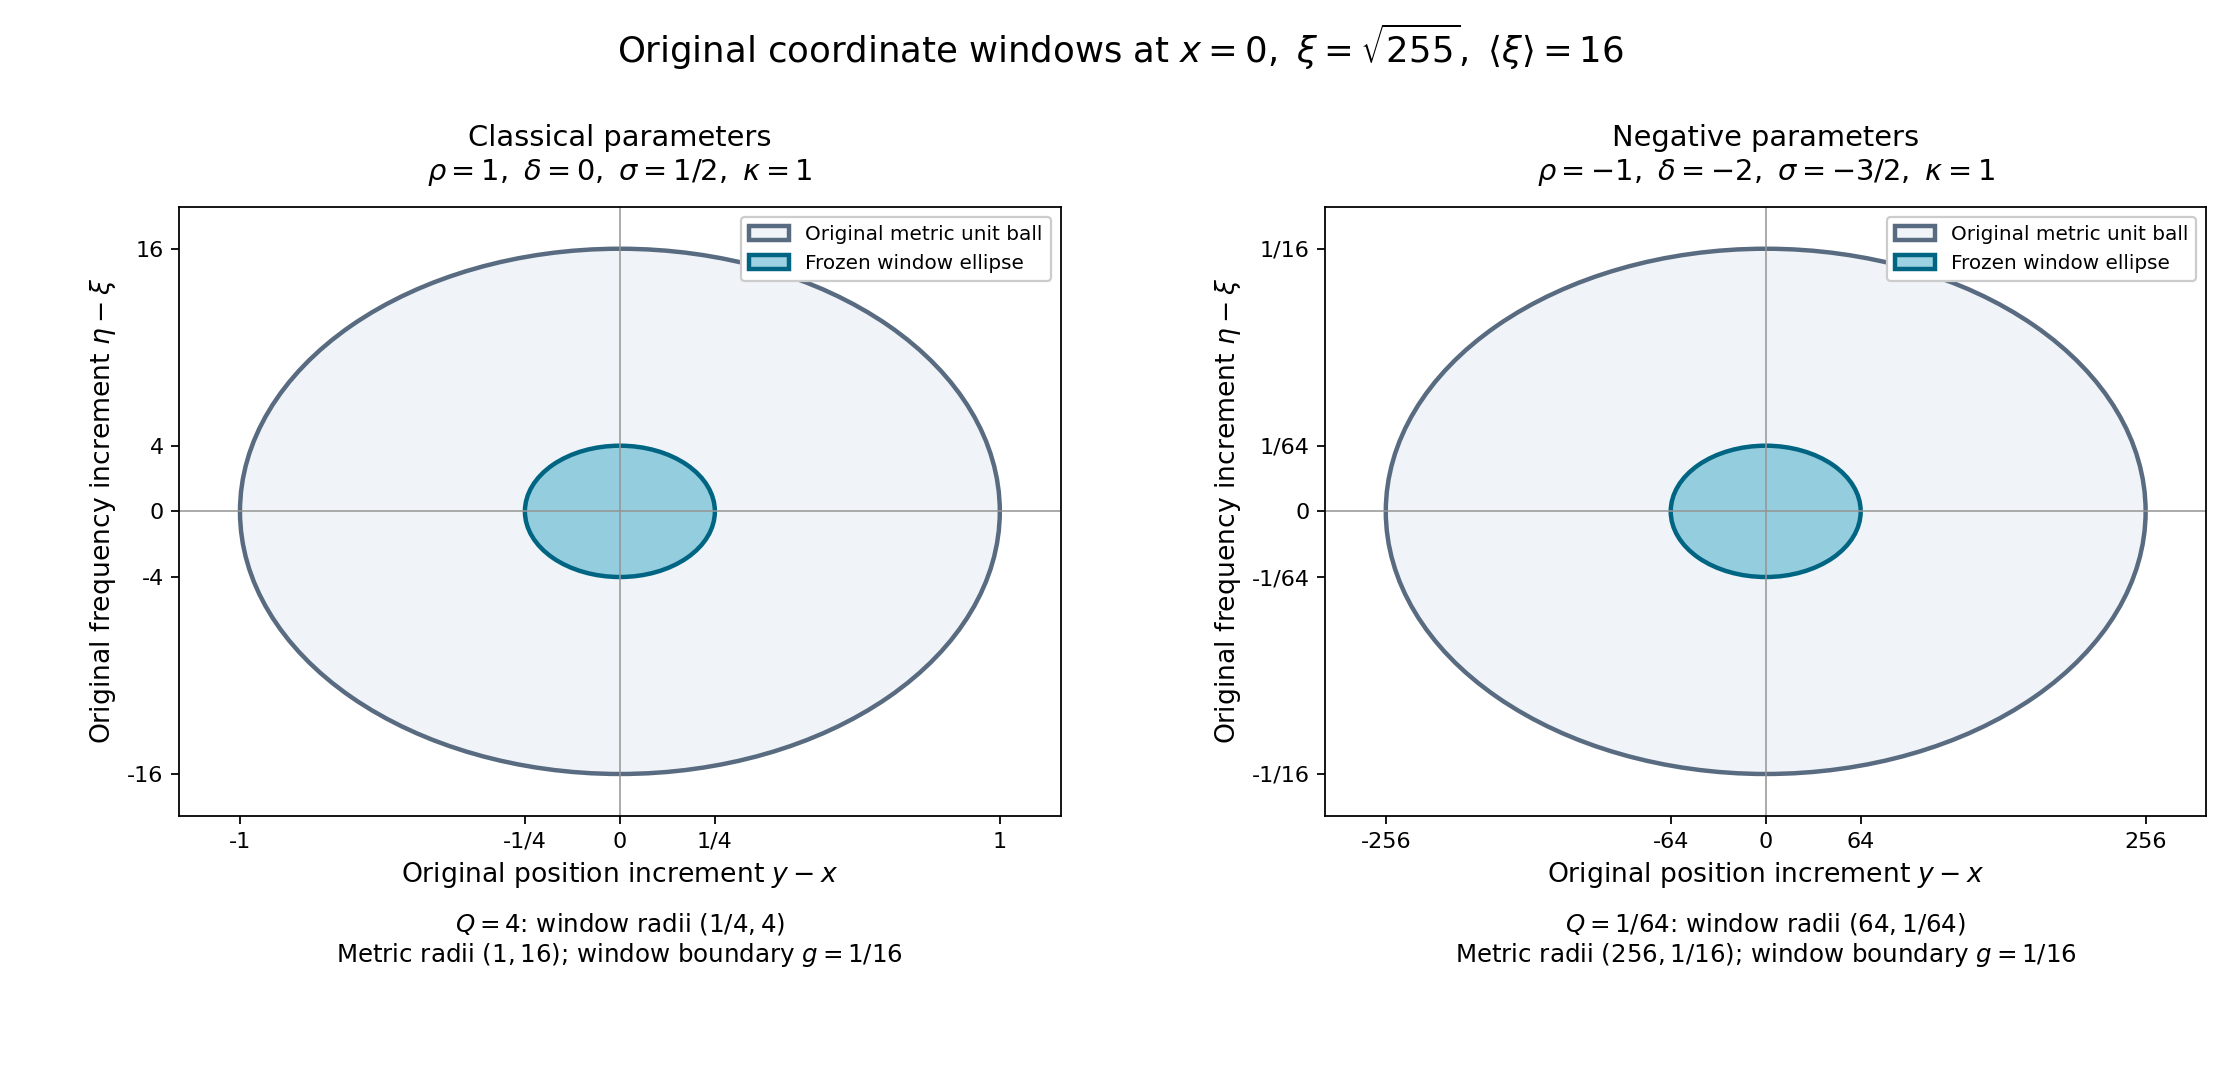
\includegraphics[keepaspectratio,alt={Two original coordinate windows inside their frozen metric ellipsoids}]{../figures/signed-window-original-coordinates.png}}
\caption{Two original coordinate windows inside their frozen metric
ellipsoids}
\end{figure}

The figure uses \(n=1\), \(x=0\), \(\xi=\sqrt{255}\), hence
\(\lambda=16\), for the classical pair \((\rho,\delta)=(1,0)\) and the
signed pair \((-1,-2)\). It draws the original tangent coordinates
\((y-x,\eta-\xi)\). The inner ellipse is
\(Q^2(y-x)^2+Q^{-2}(\eta-\xi)^2\leq1\), and the outer one is the
original frozen \(g_{(x,\xi)}\)-unit ball. Their radii are respectively
\((1/4,4)\), \((1,16)\) in the first panel and \((64,1/64)\),
\((256,1/16)\) in the second. Both inner ellipses have area \(\pi\),
both outer ellipses have area \(16\pi\), and the inner boundary has
original metric squared length \(1/16\). These follow directly by
inserting each parameter pair in (P8e), (P28e) and (P34); no coordinate
rescaling is substituted in the proof. This is a frozen window
comparison, not the support of the Schwartz seed or a claim that the
moving \(R\) in (P34) is constant. The complete moving-scale error is
proved in (P35)--(P42f). This extension has no novelty claim.

\subsection{8. Worked examples}\label{worked-examples}

\textbf{A positive symbol with a negative quadratic form.} In one
dimension let \(f(x)=2+\sin x\) and \(a(x,\xi)=f(x)\xi^2\). This is a
nonnegative classical order-two symbol. For real or complex compactly
supported smooth \(u\), integration by parts gives \[
 \operatorname{Re}\langle fD^2u,u\rangle
 =\int f|u'|^2-\frac12\int f''|u|^2
 =\int|(\sqrt f\,u)'|^2
   -\frac14\int\frac{(f')^2}{f}|u|^2.
\tag{P56}
\] Take a nonzero real \(\zeta\in C_c^\infty(\mathbb R)\) and
\(u_R(x)=\zeta(x/R)f(x)^{-1/2}\). The first term in the last expression
is \(R^{-1}\|\zeta'\|_2^2\). The second is
\(-\tfrac14\int ((f'/f)(x))^2\zeta(x/R)^2dx\), which is a negative
constant times \(R\), up to \(O(1)\). To justify that last assertion,
subtract the positive mean of the smooth periodic function \((f'/f)^2\).
Its zero-mean part has a bounded periodic primitive; one integration by
parts bounds its integral against \(\zeta(x/R)^2\) by a constant
independent of \(R\). Thus the quadratic form is negative for all
sufficiently large \(R\). The positivity of \(a\) alone did not remove
the derivative term in (P56).

\textbf{An infinite-rank positive coefficient.} Let \(H=L^2(0,1)\), and
let \(A\) be multiplication by \(1+t\). For a nonnegative scalar
\(b\in S^{2m+\kappa}_{\rho,\delta}\), the symbol \(a(x,\xi)=b(x,\xi)A\)
satisfies (P44), and (P45) applies to \(H\)-valued Schwartz functions.
The coefficient \(A\) is not a norm limit of finite-rank operators: for
every finite-rank \(F\), choose a unit vector in its kernel, obtaining
\(\|(A-F)v\|=\|Av\|\geq1\). The proof by scalar probes still applies to
this coefficient exactly.

\textbf{Equal derivative costs.} Choose a smooth annular cutoff \(\chi\)
and a scalar \(h\in C_b^\infty(\mathbb R^n)\), both nonnegative. For
\(0<r<1\), a dyadic sum
\(a(x,\xi)=\sum_{j\geq1}\chi(2^{-j}\xi)h(2^{jr}x)\) belongs to
\(S^0_{r,r}\): each point meets finitely many frequency annuli,
frequency derivatives cost at most \(2^{-j}\leq C2^{-jr}\), and position
derivatives cost \(2^{jr}\). Its boundedness follows from (P14). The
moving scale in (P28) is \(\langle\eta\rangle^r\), and the Taylor
increment in (P39) is of order one. This example makes visible why no
decreasing order was produced at equality, even though an operator bound
still holds.

\subsection{9. Exercises and solutions}\label{exercises-and-solutions}

\textbf{1. Why impose evenness on the seed?} Suppose an arbitrary
Schwartz kernel has total mass one but a nonzero first frequency moment.
Determine the leading order of its averaging error for classical symbols
at scale \(q=\langle\eta\rangle^{1/2}\).

\textbf{Solution.} At frozen scale use the kernel coordinates
\(z=Q(x-y)\), \(\theta=(\xi-\eta)/Q\). Before the scale correction, the
linear frequency Taylor term is
\(-Q\partial_{\xi_j}b\int\theta_jv(z,\theta)\,dz\,d\theta\). For
\(b\in S^r\) its possible size is
\(\lambda^{1/2}\lambda^{r-1}=\lambda^{r-1/2}\). The first position
moment has the same possible order
\(Q^{-1}\partial_{x_j}b=O(\lambda^{r-1/2})\). These are larger than the
desired \(\lambda^{r-1}\). Evenness eliminates both fixed first moments.
It also eliminates the first correction to the zeroth moment,
\(-\nabla q(\xi)\cdot\int\theta\mathcal L v\), which would otherwise
again have size \(\lambda^{-1/2}\). Thus normalization alone is
insufficient; two different uses of parity are needed.

\textbf{2. Choose the window.} For a symbol in \(S^r_{\rho,\delta}\),
suppose a phase-space cell has position radius \(\lambda^{-s}\) and
frequency radius \(\lambda^s\). Find the value of \(s\) that maximizes
the smaller of the two Taylor gains.

\textbf{Solution.} A position increment has gain \(s-\delta\); a
frequency increment has gain \(\rho-s\). Their minimum increases up to
their intersection and decreases afterwards. Hence the optimum is
\(s=(\rho+\delta)/2\), with common gain \((\rho-\delta)/2\). Quadratic
Taylor terms then have gain \(\rho-\delta\). The variation of the chosen
window contributes an additional factor \(\lambda^{s-1}\), which is no
larger than \(\lambda^{-(\rho-\delta)/2}\) precisely when \(\rho\leq1\).
This recovers both the balanced scale and the parameter condition used
in (P40).

\textbf{3. Check the distributional transpose on a first-order
operator.} In one dimension take \(a(x,\xi)=A(x)\xi\), where
\(A(x):B_1\to B_2\) is smooth with bounded derivatives. Compute the
bilinear transpose acting on tests, including its zeroth-order term.

\textbf{Solution.} Direct integration by parts in
\(\int\langle A D u,v\rangle dx\) gives \(-D(A^{\mathrm t}v)\). Thus the
transpose is \(-A^{\mathrm t}D+i(A^{\mathrm t})'\), acting from \(B_2'\)
to \(B_1'\). In (P11), \(c(x,\xi)=-A(x)^{\mathrm t}\xi\). The zeroth
term is \(-A^{\mathrm t}\xi\); the first correction is
\(\partial_\xi D_xc=i(A^{\mathrm t})'\), and all higher terms vanish.
The two calculations agree. This test detects both the reflected
frequency and the factor of \(i\).

\textbf{4. Track a shrinking high-frequency support.} Let \(a\) range
over a bounded subset of \(S^0\) and vanish for
\(|\xi|<\varepsilon^{-1}\). Prove that \(a/\varepsilon\) is uniformly
bounded in \(S^1\). Explain why ordinary order-zero boundedness applied
to \(a\) cannot by itself yield an \(O(\varepsilon)\) lower error.

\textbf{Solution.} For each \(\alpha,\beta\), the required weighted norm
is
\(\sup\varepsilon^{-1}\langle\xi\rangle^{-1+|\alpha|}\|\partial_\xi^\alpha\partial_x^\beta a\|\).
It is zero inside the open ball and bounded by the original order-zero
seminorm outside it, because
\(\varepsilon^{-1}\langle\xi\rangle^{-1}\leq1\). At the boundary the
same estimate holds by smoothness. In contrast, the order-zero seminorms
of \(a\) need not tend to zero: a cutoff that equals one sufficiently
far out has supremum one for every \(\varepsilon\). Ordinary boundedness
would give only a fixed lower bound by the operator norm. Positivity and
the order-one estimate for \(a/\varepsilon\) are what supply (P51).

\textbf{5. Locate the square-root residual.} Explain why the final power
in (P48) is \(\langle\xi\rangle^{1/2}\), and whether it follows merely
from the assertion \(a_0\in S^1\).

\textbf{Solution.} With the classical balanced window, each scaled
increment in a third-order Taylor remainder costs \(\lambda^{-1/2}\). An
order-two input therefore leaves \(\lambda^{2-3/2}=\lambda^{1/2}\). The
degree-zero, degree-one and degree-two terms were retained as actual
pointwise derivatives, with coefficients \(\lambda^{|\alpha|-1}\). This
is why the residual has that particular power. Membership in \(S^1\)
alone supplies only \(O(\lambda)\) and gives no decomposition into those
low derivatives and a smaller residual. Higher seminorms of the original
symbol control the residual constant.

\textbf{6. Which part is Hilbertian?} Does the proof establish the same
\(L^2\) and positivity results for all reflexive Banach spaces? Identify
exactly which constructions survive without a Hilbert structure.

\textbf{Solution.} Norm-valued Schwartz and symbol estimates, the
Bochner integrals, the vector-distribution description (P2)--(P4), the
transpose on Banach duals, and the ordered products and all
differentiated remainders in (P8)--(P12) survive for reflexive Banach
coefficient spaces. Equation (P13) requires the Hilbert adjoint and a
Hilbert structure. The moment lemma (P33) is Banach-valued too. The
\(L^2\) argument uses Hilbert-valued Plancherel and the packet isometry.
The positivity statement additionally uses a Hermitian quadratic form
and the operator ordering \(A\geq0\) in (P27). Those are extra
structures, so the claimed Banach calculus must not be read as a Banach
\(L^2\) boundedness or positivity theorem. Reflexivity resolves the dual
target in (P2); it does not substitute for a Hilbert norm.

\subsection{Further questions}\label{further-questions}

The moving-window proof here uses the explicit scale in (P28). Lerner's
metric treatment gives Wick positivity and a lower bound for arbitrary
Hilbert coefficients in broader metric geometry, while the calculation
here identifies the particular moving-window error (P48). Dereziński's
fixed semiclassical scale supplies a related comparison, with different
differentiated scale dependence.

Further work can ask which second-order moment tensors are attainable by
a normalized positive seed and how constants vary with the window
family. The stronger scalar Fefferman--Phong estimate needs a separate
argument; it does not follow from the operator-valued estimate (P48).
General admissible metrics likewise need their own localization and
summation proofs.

\subsection{References}\label{references}

\begin{itemize}
\tightlist
\item
  Nicolas Lerner,
  \href{https://webusers.imj-prg.fr/~nicolas.lerner/ch2booklerner.pdf}{Metrics
  on the Phase Space and Non-Selfadjoint Operators, chapter 2}, §2.4 and
  Theorem 2.5.4.
\item
  Jan Dereziński,
  \href{https://www.fuw.edu.pl/~derezins/quantize.pdf}{Introduction to
  Quantization}, version dated 19 August 2026, §4.2 and Lemma
  10.4--Theorem 10.6.
\end{itemize}

\end{document}
